%\documentclass[fleqn]{article}
\documentclass[a4paper,12pt,twoside,openright]{report}
\def\authorname{Michael Buch\xspace}
\def\authorcollege{Queens' College\xspace}
\def\authoremail{mb2244@cam.ac.uk}
\def\dissertationtitle{Collapsing heterogeneous towers of interpreters}
\def\wordcount{0}

\usepackage{epsfig,parskip,tabularx,xspace}

\usepackage[inline]{enumitem} % inline numbered lists
\usepackage[left=2cm,right=2cm]{geometry}
\usepackage{verbatim} % for comments
\usepackage{graphicx}
\usepackage{amsmath}
\usepackage{amssymb}
\usepackage[tdiagram]{semantic}
\usepackage{amsthm}
\usepackage{setspace}
\usepackage{textcomp}
\usepackage{txfonts}
%\usepackage{tikz}
%\usetikzlibrary{matrix}
\usepackage{booktabs}

% For subfigures
\usepackage{caption}
\usepackage{subcaption}

% Enumerate without spaces in between items
\newenvironment{tight_enumerate}{
\begin{enumerate}
  \setlength{\itemsep}{0pt}
  \setlength{\parskip}{0pt}
}{\end{enumerate}}

% For table formatting
\usepackage{makecell}
\usepackage{multirow}
\renewcommand\theadfont{\bfseries}

\theoremstyle{definition}
\newtheorem{definition}{Definition}[section]
\newcommand{\ts}{\textquotesingle}

\newcommand{\mslang}{$\lambda_{\uparrow\downarrow}$}
\newcommand{\mslangStar}{$\lambda_{\uparrow\downarrow}^*$}
\newcommand{\mevl}{$M_{e}$}
\newcommand{\secdlisp}{SecdLisp}

\usepackage{stmaryrd}
\usepackage{hyperref}
\hypersetup{
    colorlinks=true,
    linkcolor=blue,
    filecolor=magenta,
    urlcolor=cyan,
}
\urlstyle{same}

% Code style:
\usepackage{minted}
%\RecustomVerbatimEnvironment{Verbatim}{BVerbatim}{} % For centering markup
%\renewcommand{\figurename}{Listing}
\usemintedstyle{vs}

% For Word Count:
\newcommand{\detailtexcount}[1]{%
  \immediate\write18{texcount -merge -sum -q #1.tex lit_review.bbl > #1.wcdetail }%
  \verbatiminput{#1.wcdetail}%
}
 
\newcommand{\quickwordcount}[1]{%
  \immediate\write18{texcount -1 -sum -merge -q #1.tex lit_review.bbl > #1-words.sum }%
  \input{#1-words.sum} words%
}
 
\newcommand{\quickcharcount}[1]{%
  \immediate\write18{texcount -1 -sum -merge -char -q #1.tex lit_review.bbl > #1-chars.sum }%
  \input{#1-chars.sum} characters (not including spaces)%
}

% Section style
\setcounter{tocdepth}{3}
\setcounter{secnumdepth}{3}
\renewcommand\thesection{\arabic{section}}
\renewcommand\thesubsection{\thesection.\arabic{subsection}}
\renewcommand\thesubsubsection{\thesection.\arabic{subsection}.\arabic{subsubsection}}

\begin{document}
\pagestyle{empty}
\singlespacing

%%TC:ignore
% title page information
\begin{titlepage} 

\begin{center}
\noindent
\huge
\dissertationtitle \\
\vspace*{\stretch{1}}
\end{center}

\begin{center}
\noindent
\huge
\authorname \\
\Large
\authorcollege      \\[24pt]

\includegraphics{CUni3.eps}
\end{center}

\vspace{24pt} 

\begin{center}
\noindent
\large
{\it A dissertation submitted to the University of Cambridge \\ 
in partial fulfilment of the requirements for the degree of \\ 
Master of Philosophy in Advanced Computer Science} 
\vspace*{\stretch{1}}
\end{center}

\begin{center}
\noindent
University of Cambridge \\
Computer Laboratory     \\
William Gates Building  \\
15 JJ Thomson Avenue    \\
Cambridge CB3 0FD       \\
{\sc United Kingdom}    \\
\end{center}

\begin{center}
\noindent
Email: \authoremail \\
\end{center}

\begin{center}
\noindent
\today
\end{center}

\end{titlepage} 

\newpage
\vspace*{\fill}

%\onehalfspacing
%\newpage
{\Huge \bf Declaration}

\vspace{24pt} 

I \authorname of \authorcollege, being a candidate for the M.Phil in
Advanced Computer Science, hereby declare that this report and the
work described in it are my own work, unaided except as may be
specified below, and that the report does not contain material that
has already been used to any substantial extent for a comparable
purpose.

\vspace{24pt}
Total word count: \wordcount

\vspace{60pt}
\textbf{Signed}: Michael Buch

\vspace{12pt}
\textbf{Date}: 10th June 2019


\vfill

This dissertation is copyright \copyright 2019 \authorname. 
\\
All trademarks used in this dissertation are hereby acknowledged.



\newpage
\vspace*{\fill}

%\onehalfspacing
%\newpage
{\Huge \bf Acknowledgements}

\vspace{24pt} 
I would like to thank my supervisors, Dr. Nada Amin and Prof. Alan Mycroft, for their advice and continuous feedback throughout this work. In my regular discussions with Prof. Mycroft he helped me contextualize my thoughts and provided out-of-the-box ideas that formed the basis for much of the work I chose to pursue during the course of my thesis. His meticulous attention to detail and emphasis on clear and concise explanations were of great assistance in structuring and writing my dissertation.

My project progress and understanding of fundamental topics in partial evaluation would not have been possible without the great advice and patience of Dr. Amin. Not only has she helped me with tracking down bugs with incredible speed but shaped the direction of research that the project ended up taking. She assisted with the implementations and design of the tower of interpreters I describe in the report and her ideas, including the decision on which interpreters the tower consists of, helped keep my project, despite its experimental nature, on the right track.

Finally I would like to thank friends, family and the staff at the computer laboratory for the great support and fruitful discussions throughout the course of my studies and help broaden my horizon in the field of computer science.

\vfill

\newpage
\vspace*{\fill}
\singlespacing
\newpage
{\Huge \bf Abstract}
\vspace{24pt} 

A tower of interpreters is a program architecture that consists of a, conceptually infinite, sequence of interpreters each interpreting the one adjacent to it. Towers of interpreters in literature are synonymous with reflective towers and provide a tractable method with which to reason about reflection and design reflective languages. The overhead induced by additional layers of evaluation can be optimized away using a program specialization technique called \textit{partial evaluation}, a process which previous work has termed \textit{collapsing of towers of interpreters}. However, work on reflective towers rarely considered the implications and applicability of associated optimization techniques on practical settings in which the presence of redundant interpretation is commonplace. Our work recontextualizes prior work on reflective towers and the their collapse to \textit{heterogenous} configurations in which individual interpreters lack reflection, meta-circularity and homogeneity of data representation. First we demonstrate the construction of an experimental heterogeneous tower. Then we show evidence to support the hypothesis discussed in previous work that staging at different levels in the tower affects the optimality of the residual program. We identify obstacles that occur during the implementation of our experimental tower and the corresponding collapse procedure driven by \textit{type-directed partial evaluation (TDPE)}. As part of our tower we implement and stage a SECD abstract machine using TDPE which required the modification of its small-step semantics to support a TDPE-style reification operator and ensure termination of static reduction by normalization in the presence of recursive calls. Two core challenges we faced and provide approaches to are
\begin{enumerate*}[label=(\arabic*)]
    \item in the absence of meta-circularity binding-time information has to be passed through all interpreters in a tower for optimal residualization
    \item due to the differences in the partial evaluator's and individual interpreters' representations of closures, we need a method of transforming between the two
\end{enumerate*}.

\newpage
\vspace*{\fill}

%%TC:endignore

\pagenumbering{roman}
\setcounter{page}{0}
\pagestyle{plain}
\tableofcontents
%\listoffigures
%\listoftables

\onehalfspacing
\pagenumbering{arabic}

%TODO redraw tombstone diagarm using semantic pkg
%\begin{picture}(220,75)(0,-35)
%\put(10,0){\interpreter{S,L’}}
%\put(110,0){\program{P,\compiler{C,\machine{M},\program{P,M}}}}
%\end{picture}

%%TC:ignore
\quickwordcount{lit_review} (out of 15000)
%\quickcharcount{lit_review}
%\detailtexcount{lit_review}
%%TC:endignore

\section{Introduction}
%Towers are ...
Towers of interpreters are a program architecture which consists of sequences of interpreters where each interpreter is interpreted by an adjacent interpreter in the tower. One of the earliest mentions of such architectures in literature is a language extension to LISP called 3-LISP \cite{smith1984reflection} introduced by Smith. The treatment of programs as data is a core concept in the LISP family of languages and enables convenient implementations of LISP interpreters written in LISP themselves.  These are known as \textit{meta-circular} interpreters. In his proposal Smith describes the notion of a reflective system, a system that is able to reason about itself, as a tower of meta-circular interpreters. By way of a, conceptually infinite, \textit{reflective tower} 3-LISP enables interpreters within the tower access the internal data structures and state of the interpreter adjacent to it. A subsequent study due to Danvy et al. \cite{danvy1988intensions} provides a systematic approach to constructing reflective towers. The authors provide a denotational semantic account of reflection and develop a language based on the reflective tower model called \textit{Blond}.

%First mentions of towers was in 3-LISP. Then Friedman developed a formal account. Black was first to mention collapsing of levels of interpretation. Finally this led to a study specifically focused on towers of interpreters in Pink
%TODO: More detailed explanations (?)
%TODO: switch order of this and next paragraph?

%TODO: bold claim: rephrase
%TODO: Asai MetaOcaml->only with respect to compiled semantics
However, with respect to a traditional model of interpretation, a conceptually infinite tower of interpreters add excessive evaluation overhead solely for the purpose of achieving reflection. In the original proposals of the reflective tower models only minimal attention was given to the imposed cost of performing new interpretation at each level of a tower. Works dating back to Sturdy's thesis on reflection \cite{sturdy1993lisp} and Danvy et al.'s language Blond \cite{danvy1988intensions} hint at partial evaluation potentially being a tool capable of removing some of this overhead by specializing interpreters with respect to the interpreters below in the tower. In his language \textit{Black} \cite{asai1996duplication}, Asai et al. uses hand-crafted partial evaluation, and in a later study MetaOcaml \cite{asai2015compiling}, to efficiently implement a reflective tower and is the earliest reference to ``collapsing'' evaluation overhead in towers of interpreters. Finally, Amin et al. introduced a language Pink \cite{amin2017collapsing} to demonstrate specifically the collapse of a tower of interpreters.

%Parallel to this branch of research towers of interpreters in practice have been encountered in practice at least as long as YACC/LEX exist as Sturdy points out in his analysis of mixed language towers.
Parallel to all the above research into reflective towers, programmers have been working with towers of interpreters to some extent dating back to the idea of language parsers. Writing a parser in an interpreted language already implies two levels of interpretation: one running the parser and another the parser itself. Other examples include interpreters for embedded domain-specific languages (DSLs) or string matchers embedded in a language both of which form towers of two levels. Advances in virtualization technology has driven increasing interest in software emulation. Viewing emulation as a form of interpretation we can consider interpreters running on virtual hardware as towers of interpreters as well.

However, these two branches of research do not overlap and work on towers of interpreters rarely studied their counterparts in production systems. It is natural to ask the question of what it would take to apply previous techniques in partial evaluation to a practical setting. This is the question Amin et al. poses in their conclusion after describing Pink \cite{amin2017collapsing} and is the starting point to our thesis.

We aim to bring previous work of removing interpretative overhead using partial evaluation to towers in practice. Our study achieves this by constructing a proof-of-concept tower of interpreters that resembles one that could occur in practice. We then experiment with collapsing it under different configurations and evaluating the resulting optimized programs. We demonstrate that given a multi-level language and a lift operator we can stage individual interpreters in a sequence of non-metacircular interpreters and effectively generate code specialized for a given program eliminating interpretative overhead in the process. Our work's contributions are:
\begin{enumerate*}[label=(\arabic*)]
	\item the development of an experimental heterogeneous tower of interpreters and a strategy for collapsing it
	\item evaluation of the effects of staging at different levels within our tower on the residual programs
	\item demonstration of issues with and potential approaches to staging abstract machines, specifically a SECD machine, using TDPE
	\item discussion of the effects that heterogeneity in towers imposes on TDPE
\end{enumerate*}.

In section \ref{sec:background} we explain potentially useful background information that cover the fundamental topics we base our experiments and discussions on. Section \ref{sec:mslang} provides an overview of the partial evaluation framework called Pink \cite{amin2017collapsing} which we use in our study. We systematically describe the process by which we create a heteregeneous tower of interpreters and incrementally collapse it in sections \ref{sec:secd} through \ref{sec:string_matcher}. Each of these sections discusses the steps we took to create a level in the tower of interpreters as shown in figure \ref{fig:tombstone}. We conclude with an evaluation of our findings followed by a discussion of potential future work in sections \ref{sec:conclusion} and \ref{sec:future} respectively.

% https://tex.stackexchange.com/questions/181366/drawing-tombstone-diagrams
% https://proglang.informatik.uni-freiburg.de/teaching/compilerbau/2004/T-diagrams.pdf
% TODO: use http://mirror.its.dal.ca/ctan/macros/latex/contrib/semantic/semantic.pdf package to draw diagram
% TODO: draw diagram for practical tower as well

\begin{figure}[htp!]
\centering
    \begin{subfigure}{0.5\linewidth}
    	\centering
    	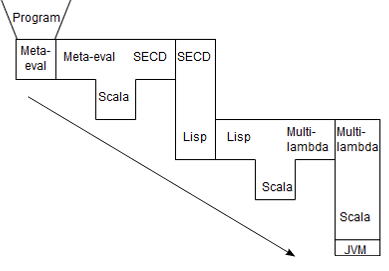
\includegraphics[scale=2]{tombstone_tower.png}
    	\caption{A tombstone diagram representation of our experimental tower}
    	\label{fig:tombstone}
    \end{subfigure}\\[1ex]
    \par\bigskip
    \begin{subfigure}{0.5\linewidth}
        \centering
        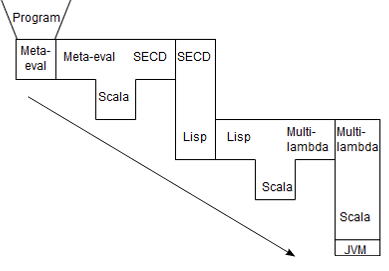
\includegraphics[scale=2]{tombstone_practical.png}
        \caption{A hypothetical tower of interpreters that serves as the model for the tower we built (shown in figure \ref{fig:tombstone}). The diagram depicts a JavaScript x86 emulator running a Python interpreter that in turn executes a python script.}
        \label{fig:tombstone_practical}
    \end{subfigure}
\caption{Comparison between the tower we develop and the one we modelled it after.}
\label{fig:tombstone_all}
\end{figure}

\section{Background}\label{sec:background}
\subsection{Interpretation and Compilation}
%Interpreters vs. compilers
An interpreter reads and directly executes instructions based on an input source program. The semantics of a programming language can be defined by the interpreter itself, in which case we call the interpreter a definitional interpreter \cite{reynolds1972definitional}.

A compiler translates a program into another representation that can subsequently be executed by some underlying machine, or interpreter. This process of translation can occur in a pipeline of an arbitrary number of stages in which a source program is transformed into intermediate representations (IR) to aid its analysis or further transformation.
%Modern optimizing compilers consist of stages in which optimization is performed on IR to improve properties of the output code such as execution speed, size or security.

%Just-In-Time (JIT) compilation is the process of compiling or recompiling pieces of a program after execution of it has begun. %The benefit of such on-demand compilation is the ability to make use of a program's execution profiles to make guide optimization %choices. Interpreters for widespread languages such as Python and Julia and frameworks such as GraalVM all make use of JIT %compilation to decrease the cost of interpretation and execute pieces of a program at native speeds. The fact that interpreters %perform compilation as well has blurred the lines between what we can term a compiler as opposed to an interpreter.

In the 1970s Futamura showed that compilers and interpreters are fundamentally related in  an elegant way by three equations also known as the Futamura projections \cite{futamura1999partial}. At its core, the three projections are based on the theory of function \textit{specialization} (or in mathematical terms \textit{projection}). Given a function $f(x,y)$, one can produce a new specialized function $f_{x}(y)$ fixed against the input $x$. In program specialization, we consider $f$ to be a program and $x$ and $y$ some inputs to said program:
\begin{align*}
    p_{x} & = \llbracket mix \rrbracket \:\: (p, x) \\
    out & = \llbracket p_{x} \rrbracket \:\: (y)
\end{align*}
where $p$ is the program being specialized, $p_{x}$ the specialized program with respect to input $x$, $mix$ is the tool that performs the specilization of $p$ and $\llbracket exp \rrbracket \:\: (arg)$ evaluates $exp$ and then applies the result to argument $arg$. In the above equations $p$ is said to have been \textit{partially evaluated}. Futamura's first projection showed that a compiler for a language $L$, $comp_{L}$, is functionally equivalent to a specializer, $mix$, for an interpreter for language $L$, $int_{L}$. In other words, partially evaluating $int_{L}$ given the source of a L-program, $src_{L}$, achieves compilation:
\begin{align*}
    target & = \llbracket mix \rrbracket \:\: (int_{L}, src_{L}) \\
           & = \llbracket comp_{L} \rrbracket \:\: (src_{L})
\end{align*}
Furthermore, \textit{self-applying} $mix$ and specializing it to an interpreter, $int_{L}$, allows one to derive a compiler from an interpreter (i.e., just a semantic description of a language):
\begin{align*}
    comp_{L} = \llbracket mix \rrbracket \:\: (mix, int_{L})
\end{align*}

A practical realization of the Futamura projections has since been an active area of research. The difficulty in their implementation is the question of \textit{how} one can specialize an interpreter and meanwhile also generate the most efficient and correct code, a question that is being explored in the design of partial evaluators to this day \cite{jones1988challenging,jones1993partial}.

\subsection{Type-Directed Partial Evluation}
%https://link.springer.com/content/pdf/10.1007%2F3-540-47018-2.pdf
Partial evaluation (PE) is a program optimization technique based on the insight that there is room in programs for statically reducing and producing a specialized and thus hopefully more efficient version of itself. A \textit{partial evaluator} determines whether operations involving inputs to specialize against can be reduced or have to be left in the program. A \textit{residual program}, is a version of the original program where as much computation as possible has been performed with the data that was available at specialization time (i.e., during run-time of the partial evaluator). The portion of data that is known at specialization time is called \textit{static} and otherwise \textit{dynamic}. For variables in the program to-be-specialized we refer to it's \textit{binding-time} as static if the data it holds during the lifetime of the program is static. Otherwise a variable's binding-time is dynamic.

The result of a \textit{binding-time analysis} is called a \textit{division} and assigns to each function and variable in a program a binding-time. A division is said to be congruent if it assures that every expression that involves dynamic data is marked as dynamic and otherwise as static. A partial evaluator being just a regular program, a problem one can run into is non-termination. A congruent division does not always guarantee termination of a PE but when it does we call the division \textit{safe}.
%In our case our division does not ensure termination but rather our implementation and special treatment of function specialization

% EXAMPLE OF CONGRUENCE AND NON-TERMINATION THAT IS APPLICABLE TO STAGED SECD
%Polyvariant binding-time analysis for applicative languages
%http://pages.cs.wisc.edu/~horwitz/CS704-NOTES/9.PARTIAL-EVALUATION.html#div

%There are two types of partial evaluation methodologies :
%\begin{itemize}
%	\item Offline partial evaluation
%	\item Online partial evaluation \cite{cook2011tutorial}
%\end{itemize}

%TODO: Pink really online? TDPE is actually an offline PE technique
In the literature we distinguish between \textit{online} and \textit{offline} partial evaluation \cite{jones1993partial} (or more recently a hybrid between the two due to Shali et al. \cite{shali2011hybrid}). Offline PE performs a BTA before it begins specialization whereas the online approach makes decisions about whether to residualize expressions once partial evaluation has begun.

Danvy realized a method of implementing a partial evaluator solely based on the ideas of normalization in the simply-typed $\lambda$-calculus called \textit{Type-Directed Partial Evaluation (TDPE)} \cite{danvy1999type}. The result is a remarkably simple methodology of implementing residualizers with a binding-time analysis that is completely driven by the types of the expressions being specialized. TDPE is built on three core concepts \cite{danvy1999type,grobauer2001second}:
%TODO: well-annotatedness
\begin{tight_enumerate}
    \item BTA produces an expression annotated with the static or dynamic binding-times such that reducing static terms yields a completely dynamic expression (i.e., permits optimal residualization)
    \item BTA should generate code that includes \textit{binding-time coercions}, which are modifications to the original terms that aid the correct classification of expressions as static
    \item Static reduction is performed by evaluation of an expression and well-formedness of the generated code is guaranteed by the implementing language's type system
\end{tight_enumerate}

Consider the example from Danvy's description of TDPE \cite{danvy1999type} in \eqref{eq:tdpe_ex1}. The aim is to annotate the function applications (denoted by $@$) and definitions with a static (overline) or dynamic (underline) binding-time.
\begin{align}
    \lambda g.\lambda d.(\lambda f.g \:@ \: (f \: @ \: d)\: @ \:f) \: @ \: \lambda a.a \label{eq:tdpe_ex1}
\end{align}

A correct binding-time could be that shown in \eqref{eq:tdpe_ex2a} because after static reduction we obtain \eqref{eq:tdpe_ex2b} which is a completely dynamic expression. However, the duplication of $f$ after reduction and a dynamic redex, $(\underline{\lambda}a.a) \: \underline{@} \: d$, could be optimized away further with a modification to the source expression (i.e., a binding-time coercion). The challenge we are faced with is that $f$ is applied statically but cannot be completely reduced because we also pass it as an argument to a dynamic expression.
\begin{figure}[hbp!]
    \begin{align}
        & \underline{\lambda g}.\underline{\lambda} d.(\overline{\lambda} f.g \: \underline{@} \: (f \: \underline{@} \: d) \: \underline{@} \: f) \: \overline{@} \: \underline{\lambda} a.a) \label{eq:tdpe_ex2a} \\
        & \triangleright \:\: \emph{\small{\text{(via static reduction)}}} \nonumber \\
        & \underline{\lambda g}.\underline{\lambda} d.(\lambda g \: \underline{@} \: ((\underline{\lambda} a.a) \: \underline{@} \: d) \: \underline{@} \: \underline{\lambda} a.a \label{eq:tdpe_ex2b}
    \end{align}
\end{figure}

Instead we can use an $\eta$-expansion to turn instances of $f$ as a higher-order value into static function applications. The resulting annotations are shown in \eqref{eq:tdpe_ex3a} and the $\eta$-expansion is highlighted in green. After static reduction we obtain the optimal expression in \eqref{eq:tdpe_ex3b} that only contains dynamic values, only a single unfolding of $f$ and no $\beta$-redexes. Danvy then generalizes the $eta$-expansion into a class of coercions that permit residualization of static values in dynamic contexts. We represent such coercions with a $\downarrow^t$ (or \textit{lift} as we use in later sections and as defined in figure \ref{fig:tdpe_rules}) which represents the conversion from a static value of type $t$ to a dynamic value. Using the coercion operator, TDPE would yield the annotation in \eqref{eq:tdpe_ex4}.

\begin{figure}[htp!]
    \begin{align}
        & \underline{\lambda g}.\underline{\lambda} d.(\overline{\lambda}f.g \: \underline{@} \: (f \: \overline{@} \: d) \: \underline{@} \: \text{\colorbox{green}{$\underline{\lambda} x.f \: \overline{@} x$}}) \: \overline{@} \: \overline{\lambda} a.a \label{eq:tdpe_ex3a} \\
        & \triangleright \:\: \emph{\small{\text{(via static reduction)}}} \nonumber \\
        & \underline{\lambda g}.\underline{\lambda} d.g \: \underline{@} \: d \: \underline{@} \: \underline{\lambda} a.a \label{eq:tdpe_ex3b}
    \end{align}
\end{figure}

\begin{figure}[htp!]
    \begin{align}
        & \underline{\lambda g}.\underline{\lambda} d.(\overline{\lambda}f.g \: \underline{@} \: (f \: \overline{@} \: d) \: \underline{@} \: \text{\colorbox{green}{(\textit{lift} $f$)}}) \: \overline{@} \: \overline{\lambda} a.a \label{eq:tdpe_ex4} \\
        & \quad \text{where we omit the first type argument to \textit{lift} for simplicity} \nonumber
    \end{align}
\end{figure}

%\begin{figure}[htp!]
%    \begin{align}
%        & \underline{\lambda g}.\underline{\lambda} d.(\overline{\lambda}f.g \: \underline{@} \: %(f \: \overline{@} \: d) \: \underline{@} \: \text{\colorbox{green}{$\downarrow^{t_{1} %\rightarrow t_{2}} f$}}) \: \overline{@} \: \overline{\lambda} a.a \label{eq:tdpe_ex4} %\\
%        & \quad \text{where $t_{1} \rightarrow t_{2}$ is the type of $f$} \nonumber
%    \end{align}
%\end{figure}

%\subsection{\texorpdfstring{$\eta$-expansion}{Lg} in TDPE}
To summarize TDPE makes use of the type system of a two-level language to direct the residualzation of expressions. The output of this lightweight BTA is an expression whose terms are annotated with dynamic or static binding times which when statically reduced yield a purely dynamic expression. Static reduction is performed through regular evaluation of the two-level language's interpreter. TDPE includes a set of operators to convert between dynamic and static terms to aid the optimality of generated code. The two classes of coercion operators are reification (also called lift) and reflection both of which are defined on product, function and literal types. Residualization is finally defined as performing annotations and binding-time coercions followed by static reduction.

As dicussed in section \ref{sec:mslang}, the Pink \cite{amin2017collapsing} partial evaluator implements most of the binding time coercions according to figure \ref{fig:tdpe_rules}'s definitions with the exception of \textit{reflect}, which is implemented using an algorithm attributed to Eijiro Sumii \cite{hatcliff2007partial} to handle order of evaluation of side-effects.
%TODO: revisit reification for recursive functions in TDPE paper
%TODO: Pink also introduces a ``run'' operator

\begin{figure}[htp!]
    \centering
    \begin{alignat}{2}
        \text{\underline{\textbf{\emph{Reification (Lifting)}}}}\nonumber \\
        \downarrow^{t} v & = \: && v \\
        \nonumber \\%
        \downarrow^{t_{1} \rightarrow t_{2}} v & = \: && \underline{\lambda} x.\downarrow^{t_{2}}(v\overline{@}(\uparrow_{t_{1}} x)) \\
        & && \quad\text{where $x$ is not a free variable in v} \nonumber \\
        \nonumber \\%
        \downarrow^{t_{1} \times t_{2}} v & = \: && \underline{cons}(\downarrow^{t_{1}} \overline{car} \, v, \downarrow^{t_{2}} \overline{cdr} \, v) \\
        \nonumber \\%
        lift & = \: && \lambda t. \lambda v. \downarrow^{t} v \\
        \nonumber \\%
        %
        \text{\underline{\textbf{\emph{Reflection}}}}\nonumber \\
        \uparrow_{t} e & = \: && e \\
        \nonumber \\%
        \uparrow_{t_{1} \rightarrow t_{2}} e & = \: && \overline{\lambda} v.\uparrow_{t_{2}}(e\underline{@}(\downarrow^{t_{1}} v)) \\
        \nonumber \\%
        \uparrow_{t_{1} \times t_{2}} e & = \: && \overline{cons}(\uparrow_{t_{1}} \underline{car} \, e, \uparrow_{t_{2}} \underline{cdr} \, e) \\
        \nonumber \\%
        reflect & = \: && \lambda t. \lambda e. \uparrow_{t} e
    \end{alignat}
    \caption{Reduction rules for reification (static to dynamic) and reflection (dynamic to static) in TDPE as defined by Danvy \cite{danvy1999type} where $t$ denotes types, $v$ denotes static values, $e$ denotes dynamic expressions. $cons/car/cdr$ correspond to the LISP functions of the same name that create a pair, reference the first element of a pair and reference the second element of a pair respectively.}
    \label{fig:tdpe_rules}
\end{figure}

%Early partial evaluators, including Jones et al.'s MIX \cite{jones1989mix}, operated exclusively on %untyped languages because it simplified binding time analysis: a single universal type could %represent all static values and would not need to care about whether BTA violated a type-system. To %broaden the applicability of partial evaluation 
%
%* binding time is automatic (or requires annotations only on inputs to program e.g. like in Pink, %which requires knowledege of how the binding-time works. TDPE only requires annotations on base %types from which product, sum and function types' binding-times can be deduced. Pink does not %necessarily have a binding time analysis step which makes it slightly more convenient for manual %annotation)
%* type-directed means we use the type of a term to guide the normalization (i.e. ``extraction %function'' is parameterized by type)
%* TDPE reuses underlying evaluator to perform static evaluation vs code generation. Traditionally %these are performed by the partial evaluator separately in the form of symbolic computation on the %source. Pink takes the former approach
%
%In \cite{danvy1999type} Danvy builts a language in ML that supports and reflection (section 1) and %then shows how partial evaluation of can be achieved using a ``normalization function'':
%%In  summary,  if  one  implements  the  two-level  lambda-calculus  as  in  Sec-tion  1.3, then %reifying  a simply typed,  closed, and completely static  higher-order  function  into  a  dynamic  %expression  automatically  yields  a  representation  of  its  normal form.  In the rest  of this %section,  we illustrate this phenomenon  with  de-compilation,  before  turning to the  %implementation  of  a normalization  function  in  ML.
%
%page 379 explains role of let-insertion
%pg 395: Our framework uses the Eijiro Sumii  approach
%
%page 388: actual description of TDPE
%"We  define  type-directed  partial  evaluation  as normalization  by  evaluation  over  ML values"
%
%page 403: benefits of NbE
%
%jones page. 103: ``The Trick''
%\cite{jones1993partial} page 113: monovariance, polyvariance, congruence in PE, just need to lift products/functions/sum types => reason we stage interpreter that way in Pink and our towers
%Reification according to TDPE (pg. 381): static to dynamic
%Reflection ": dynamic to static
%pg 380: well-annotatedness ensured my Scala's type system (static reduction cannot go wrong guaranteed by evaluation) and the type Exp (result is dynamic if result is Exp=>ensures consequence of annotation turns expression completely dynamic). " Conceptually, well-annotatedness is reduced to ML typeability and static reduction to ML evaluation"
%reflection/reification are forms of binding-time coercions
%pg. 380: "a binding-time coercion maps an expression into a new expression to ensure well-annotatedness between expressions and their contexts during static reduction. In that, binding-time coercions fulfill the same task as, e.g., subtype coercions
%pg. 381: how to coerce a closed, completely static expression into the corresponding dynamic expression. This coercion is achieved using the type-directed translation displayed in Figure 2, which can be seen to operate by "two-level eta expansion"
%
%http://web.cs.ucla.edu/~palsberg/paper/pe99.pdf pg. 2: To obtain consistency, Mix-style partial evaluators [14] coerce static values and contexts to be respectively dynamic values and dynamic contexts, when they encounter a clash. This is acceptable if source programs are first-order and values are either fully static or fully dynamic. However these coercions are excessive for programs with partially static values and contexts.
%http://web.cs.ucla.edu/~palsberg/paper/pe99.pdf and "partial Evaluation of General Parsers": "The Trick"

\subsection{\texorpdfstring{\mslang}{Lg} Overview}\label{subsec:mslang}
%TODO: revisit lift of functions (especially recursive) in Pink

%TODO: reword
Since our work is based on the multi-level language, \mslang, developed by Amin et al. \cite{amin2017collapsing} we provide a summary of the core language which is a call-by-value $\lambda$-calculus split into two evaluation contexts, one in which expressions are code and the other in which expressions normalize to values. The framework also includes a LISP front-end that translates s-expressions into terms of \mslang. We will be using this framework as the basis for our tower of interpreters. The language distinguishes between \textit{expressions}, which are terms in a \mslang{} program, and \textit{values} which represent the static output after evaluating an expression. Thus when we talk about generating code using \mslang{}, we mean \textit{values} in the language.
%TODO: 2 levels actually come from statics and dynamic. In literature overlines/underlines indicate stage but in \mslang Val vs Exp determines stage (pg. 379)

\begin{figure}
    \centering
    \begin{minted}[escapeinside=||,fontsize=\footnotesize]{scala}
// Converts Expressions (Exp) into Values (Val)
def evalms(env: Env, e: Exp): Val = e match {
    case Lit(n) => Cst(n)
    case Sym(s) => Str(s)
    case Var(n) => env(n)
    case Lam(e) => Clo(env,e)
    case Lift(e) =>
      Code(lift(evalms(env,e)))
    ...
    case If(c,a,b) =>
      evalms(env,c) match {
        case Cst(n) => 
          if (n != 0) evalms(env,a) else evalms(env,b)
        case (Code(c1)) => |\textcolor{red}{<=== Generate an if-statement if conditional is dynamic}|
          reflectc(If(c1, reifyc(evalms(env,a)), reifyc(evalms(env,b))))
      }
    ...
}
...
var stBlock: List[(Int, Exp)] = Nil
def reify(f: => Exp) = run {
    stBlock = Nil
    val last = f
    (stBlock.map(_._2) foldRight last)(Let) |\textcolor{red}{<=== Let-insertion occurs here}|
}
def reflect(s:Exp) = {
    stBlock :+= (stFresh, s)
    fresh()
}
// NBE-style 'reify' operator (semantics -> syntax)
def lift(v: Val): Exp = v match {
    case Cst(n) => // number
      Lit(n)
    case Str(s) => // string
      Sym(s)
    case Tup(Code(u),Code(v)) => reflect(Cons(u,v))
    case Clo(env2,e2) => // function
      stFun collectFirst { case (n,`env2`,`e2`) => n } match {
        case Some(n) =>
          Var(n)
        case None =>
          stFun :+= (stFresh,env2,e2)
          reflect(Lam(reify{ val Code(r) = evalms(env2:+Code(fresh()):+Code(fresh()),e2); r }))
      }
    case Code(e) => reflect(Lift(e))
}
...
    \end{minted}
    \caption{Main points of interest of the \mslang{} evaluator architecture.}
    \label{lst:evalms}
\end{figure}

Figure \ref{lst:evalms} provides an overview of the structure of \mslang{} as a partial evaluator which closely follows the description given by Danvy \cite{danvy1999type} on TDPE. Given an expression the PE evaluates terms to values while differentiating between static values (simply \texttt{Val}) and dynamic values (terms wrapped in the \texttt{Code} constructor). An expression wrapped in a \texttt{Lift} constructor gets evaluated to \texttt{Code} and appears in the residual program. 

%TODO: Eijiro Sumii implementation of TDPE
In \mslang{} the TDPE \textit{reify} operation is called \textit{lift}. The function converts semantics of an expression to its syntax and thus can be said to generate code (i.e., terms of \mslang). The fact that code generation of expressions can be guided using this single operator, whose semantics closely resemble expression annotation, is attractive for converting interpreters into translators. A user of \mslang{} can stage an interpreter by annotating it's source provided the possibility of changing the interpreter's internals and enough knowledge of its semantics.

We make use of the notion of \textit{stage-polymorphism} introduced by Offenbeck et al. \cite{ofenbeck2017staging} to support two modes of operation:
\begin{enumerate*}[label=(\arabic*)]
	\item regular evaluation
	\item generation and subsequent execution of \mslang{} terms
\end{enumerate*}.
Stage-polymorphism allows abstraction over how many stages an evaluation is performed with. This is achieved by operators that are polymorphic over what stage they operate on and is simply implemented as shown in figure \ref{lst:stage_poly_ex}. Whenever the \textit{lift} operator is now used in the \textit{interpreter} or \textit{compiler} it will cause \textit{evalms} to either evaluate or generate code respectively.

\begin{figure}[ht]
\centering
\begin{minted}{lisp}
(let interpreter (let maybe-lift (lambda (x) x) (...)))
(let compiler (let maybe-lift (lambda (x) (lift x)) (...)))
\end{minted}
\caption{``Stage-polymorphism'' implementation from Amin et al.'s Pink \cite{amin2017collapsing}}
\label{lst:stage_poly_ex}
\end{figure}

%TODO: recipe is actually mentioned in pg. 377 (https://link.springer.com/content/pdf/10.1007%2F3-540-47018-2.pdf)
An advantage of TDPE and why \mslang{} serves as an appropriate candidate PE in our experiments is that it requires no additional dedicated static analysis tools to perform its residualization, keeping complexity at a minimum. Given an interpreter we can stage it by following Amin et al.'s \cite{amin2017collapsing} recipe: lift all terminal values an interpreter returns. Once the returned values are dynamic, any operation that includes them is also marked dynamic and will occur in the residual program.

%TODO: explain SECD such that code snippets in later sections are understandable to new reader
\subsection{Abstract Machines}
%The full small-step semantics of the machine are given in APPENDIX and figures FIGURES demonstrate examples of how the machine operates.
The SECD machine due to Landin \cite{landin1964mechanical} is a well-studied stack-based abstract machine initially developed in order to provide a model for evaluation of terms in the $\lambda$-calculus. All operations on the original SECD machine are performed on four registers: stack (S), environment (E), control (C), dump (D). \textit{C} holds a list of instructions that should be executed. \textit{E} stores free-variables, function arguments, function return values and functions themselves. The \textit{S} register stores results of function-local operations and the \textit{D} register is used to save and restore state in the machine when performing control flow operations. A step function makes sure the machine progresses by reading next instructions and operands from the remaining entries in the control register and terminates at a STOP or WRITEC instruction, at which point the machine returns all values or a single value from the S-register respectively.

\section{Heterogeneity}\label{sec:heterogeneity}
A central part of our study revolves around the notion of heterogeneous towers. Prior work on towers of interpreters that inspired some these concepts includes Sturdy's work on the Platypus language framework that provided a mixed-language interpreter built from a reflective tower \cite{sturdy1993lisp}, Jones et al.'s Mix partial evaluator \cite{jones1989mix} in which systems consisting of multiple levels of interpreters could be partially evaluated and Amin et al.'s study of collapsing towers of interpreters in which the authors present a technique for turning systems of meta-circular interpreters into one-pass compilers. We continue from where the latter left of, namely the question of how one might achieve the effect of compiling multiple interpreters in heterogeneous settings. Our definition of \textit{heterogeneous} is as follows:
\theoremstyle{definition}
\begin{definition}
	Towers of interpreters are systems of interpreters, $I_0, I_1, ..., I_n$ where $n \in \mathbb R_{\ge 0}$ and $I_n$ determines an interpreter at level $n$ interpreted by $I_{n-1}$, written in language $L$ such that $L_{I_n}$ is the language interpreter $I_n$ is written in.
\end{definition}
%TODO: provide diagram for the above definition

%A level here is analogous to an instance of an interpreter within the tower and as such level $n$ implies $I_n$ if not mentioned explicitly otherwise.

\begin{definition}
    \label{def:het}
	Heterogeneous towers of interpreters are towers which exhibit following properties:
	\begin{enumerate}
		\item For any two levels $n, m \in \mathbb R_{\ge 0}, L_{I_n} \not\equiv L_{I_m}$
		\item For any two levels $n, m \in \mathbb R_{\ge 0}, L_{I_n} \not\blacktriangleleft L_{I_m}$, where $\blacktriangleleft$ implies access to the left-hand side interpreter's state and $m \ge n$
		\item For any two adjacent interpreters used in the tower, $I_{n}$ and $I_{n-1}$, the operational semantics \textit{or} the representation of data is different between the two
	\end{enumerate}
\end{definition}

\subsection{Absence of: Meta-circularity}
The first constraint imposed by definition \ref{def:het} is that of necessarily mixed languages between levels of a tower. A practical challenge this poses for partial evaluators is the inability to reuse language facilities between levels of a tower. This also implies that one cannot define reflection and reification procedures as in 3-LISP \cite{smith1984reflection}, Blond \cite{danvy1988intensions}, Black \cite{asai1996duplication} or Pink \cite{amin2017collapsing}.

\subsection{Absence of: Reflection}
The ability to introspect and change the state of an interpreter during execution is a tool reflective languages use for implementation of debuggers, tracers or even language features. Reflection in reflective towers implies the ability to modify an interpreter's interpreter. With reflection, however, programs can begin to become difficult to reason about and preventive measures for potentially destructive operations on a running interpreter's semantics introduces overhead. Towers that we are interested in rarely provide reflective capabilities in every, or even a single, of its interpreters.

\subsection{Semantic Gap and Mixed Language Systems}
An early mention of non-reflective and non-metacircular towers was provided in the first step of Danvy et al.'s denotational description of the reflective tower model \cite{danvy1988intensions}. The authors explored the idea of having different denotations for data at every level of the tower. However, since it was not the focus of their study, the potential consequences were not further investigated but serves as the motivation for point three of definition \ref{def:het}. We call the difference in operational semantics or data representation between two interpreters a \textit{semantic gap}.

%TODO: reword
An extensive look at mixed languages in reflective towers was performed in chapter 5 of Sturdy's thesis \cite{sturdy1993lisp} where he highlighted the importance of supporting a mixture of languages within his interpretation framework and provided examples of multi-layer systems such as invocation of the UNIX shell through Make a script. Sturdy goes on to introduce into his framework support for mixed languages that transform to a LISP parse tree to fit the reflective tower model. We remove the requirement of reflectivity and argue that this provides a convenient way of collapsing, through partial evaluation a mixed level tower of interpreters. While Sturdy's framework \textit{Platypus} is a reflective interpretation of mixed languages, we construct a non-reflective tower consisting of mixed languages.

One of our motivations stems from the realization that systems consisting of several layers of interpretation can feasibly be constructed. A hypothetical tower of interpreters that served as a model for the one we built throughout our work was described in Amin et al.'s paper on collapsing towers \cite{amin2017collapsing} and is depicted as a tombstone diagram in figure \ref{fig:tombstone_practical}. As a comparison our diagram is shown in \ref{fig:tombstone}. We replace the x86 emulator with a SECD abstract machine interpreter and Python with our own functional toy language, \textit{Meta-eval}. Multi-lambda is the partial evaluator and multi-level core language from Pink \cite{amin2017collapsing}. Although here the tower grows upwards and to the left, this need not be. The compilers, or \textit{translators}, from Meta-eval to SECD and from Lisp to Multi-lambda have been implemented in Scala purely for simplicity. To realize a completely vertical tower (i.e., consisting of interpreters only), our Lisp to Multi-lambda translator, which converts LISP source to Scala ASTs, could be ommitted letting the base evaluator evaluate s-expressions directly. Similarly, the Meta-eval to SECD compiler could be implemented in SECD instructions itself. However, we argue that the presence of compilation layers in our experimental tower resembles a setting in practice more closely and adds some insightful challenges to our experiments.

\section{Recipe to Collapsing Towers}
In this section we describe the methodology that Pink uses to construct and collapse towers and then discuss changes that have to be considered when applying it to a heterogeneous setting.

\subsection{TDPE and Staging a Definitional Interpreter}\label{subsec:stage_def_interp}
Pink defines a multi-level language that differentiates between static and dynamic values. This is essential to express binding-time information. Then the lift and reflect operators are implemented such that BTA can coerce static to dynamic values or vice versa respectively.

In his original description of TDPE  Danvy \cite{danvy1999type} showed that we can use above tools to residualize a definitional interpreter with respect to a source program. Pink demonstrates how to stage such an interpreter by wrapping all literal, function and product types in calls to a TDPE-style lift (i.e., reify) operator. Additionally, Pink introduces the concept of \textit{binding-time agnostic staging}. Here, the same definition of an interpreter can be used to residualize or simply evaluate a program. In reference to Pink, \textit{staging an interpreter} means lifting types as described above but also activating \textit{code generation mode}, a detail we use in the next section.
%TODO: effect of wrapping user-level values on BTA

\subsection{Construct and the Collapse Tower}
A tower can then be constructed using a, potentially infinite, set of meta-circular interpreters each interpreting the next level in the tower. The key benefit of meta-circularity and the basis of collapsing the tower is that the \textit{lift} built-in defined in the base evaluator is accessible to each interpreter. We can then stage the user-most interpreter (i.e., the interpreter running the program provided by the user), as described in section \ref{subsec:stage_def_interp}. Although previous work did not provide an insight into the exact effect of staging at different levels in the tower, an intuitive reason we stage at the top-most level is that we want to eliminate as much interpretative overhead as possible which is achieved by collapsing the maximal set of interpreters in the tower. In our experimental tower in sections \ref{sec:mslang} to \ref{sec:string_matcher} we provide evidence to support this claim.

%TODO: show diagram (tower.ppt)
When we now execute the tower (i.e., invoking the partial evaluator at the base) only the top-most evaluator residualizes while all others evaluate. Because of meta-circularity, instead of evaluating a user-value it is now being lifted at all stages essentially propagating binding-time information from top-most interpreter to the base PE. At the last interpreter above the base evaluator, the lift now dispatches to the actual reify operation as specified by TDPE. Effectively after residualization the generated program will only include the values staged at the top-most interpreter while the rest of the tower was reduced at specialization time since they were not evaluated in code-generation mode.

\subsection{Effect of Heterogeneity}
%TODO: explain using diagram
In mixed-language towers a \textit{lift} operation is not necessarily available to all interpreters unless explicitly provided at that level. Hence, one approach to propagating binding-time information in heterogeneous towers is to implement a built-in lift at all levels below the interpreter that should be staged. As we discuss in more detail in section \ref{subsec:secd_staged}, the implementation of lift may require us to transform the representation of closures, pairs or other constructs which the lift at the base expects.

Additionally, the TDPE residualization algorithm uses evaluation of expressions to drive its BTA and static reductions. While a definitional interpreter can be staged using TDPE by simply lifting user-values it returns, the process of staging an abstract machine, as we show in \ref{subsec:secd_staged}, requires careful design of its division rules and consideration at which locations to lift. Representation of closures can cause issues with non-termination if there is no inherent distinction between regular and recursive function definitions. To avoid these issues one can transform the representation of closures to fit the underlying lift operation's interface and use tags on closures that signal the PE when to terminate in the unfolding of recursive function calls.
%tricks involve eta-expansion again

%challenges of staging SECD
%TODO: tower is not framework
%Describe results found: difficulties in heterogeneous setting
%Can be done in multiple ways: can either turn into compiler or let lift sift through
%Describe essence

%TODO: extend using below snippets
%The mix partial evaluation framework \cite{jones1989mix}, Jones et al. demonstrate the PE of a simple interpreter into a language called Mixwell developed by the authors. This is similar in spirit to our framework except it is smaller in height. (section 5 of the paper \cite{jones1989mix}). also mentions removal of layers of meta-interpretation in its conclusion

%Partial Evaluation of Machine Code

%Put together, the three properties imposed by definition \ref{def:het} encourage a generalized solution irregardless of the language or structure of the tower at hand.

\section{Construction of an Experimental Heterogeneous Tower}
\subsection{Level 1: \texorpdfstring{\mslang}{Lg}}\label{sec:mslang}
%Stage only user-most interpreter (we investigate configurations in this thesis): \textit{wire tower} such that the \textbf{staging commands in $L_{n}$ are interpreted directly in terms of staging commands in $L_{0}$} i.e. staging commands pass through all other layers handing down commands to layers below without performing any staging commands

%In partial evaluation terms, the configurations, i.e. set of run-time computational states, is stored in stBlock while the division, i.e. denotation of static vs dynamic values
The first level in our tower is the evaluator for \mslang{} which we mostly take from the way it was defined in Pink. It serves as our partial evaluator and generates \mslang{} terms, in A-Normal Form \cite{flanagan1993essence}, given LISP expressions through its front-end.

To reduce the amount of generated code we add logic within \mslang's \textit{reflect} that reduces purely static expressions. Reducible expressions include arithmetic and list access operations. We refer to these in later sections as \textit{smart constructors} and they aid in normalizing static expressions that the division (described in section \ref{subsec:secd_staged}) does not permit. These are shown in an excerpt of \mslang's definitional interpreter in figure \ref{lst:mslang_interp}.

\begin{figure}
    \centering
    \begin{minted}[escapeinside=||]{scala}
def reflect(s:Exp) = {
    ...
    case _ =>
        s match {
          |\colorbox{green}{case Fst(Cons(a, b)) => a}|
          |\colorbox{green}{case Snd(Cons(a, b)) => b}|
          |\colorbox{green}{case Plus(Lit(a), Lit(b)) => Lit(a + b)}|
          |\colorbox{green}{case Minus(Lit(a), Lit(b)) => Lit(a - b)}|
          |\colorbox{green}{case Times(Lit(a), Lit(b)) => Lit(a * b)}|
          case _ =>
            stBlock :+= (stFresh, s)
            fresh()
        }
}
    \end{minted}
    \caption{\textit{Smart constructors} (highlighted in green) in \mslang's \textit{reflect}}
    \label{lst:mslang_interp}
\end{figure}

% Power of a dedicated "lift" instruction -> turns interpreter into compiler with ease and can, as we demonstrated, even remove a translation layer (metaeval -> SECD translator)

\subsection{Level 2: SECD}\label{sec:secd}
Our reasoning behind choosing the SECD abstract machine as one of our levels is three-fold:
\begin{enumerate}
	\item \textbf{Maturity}: SECD was the first abstract machine of its kind developed by Landin in 1964 \cite{landin1964mechanical}. Since then it has thoroughly been studied and documented \cite{danvy2004rational,ramsdell1999tail,henderson1980functional} making it a strong foundation to build on.
	%SECD doesn't have first-class functions
	\item \textbf{Large Semantic Gap}: A central part of our definition of heterogeneity is that languages that adjacent interpreters interpret are significantly different from each other (see section \ref{sec:heterogeneity}). In the case of SECD's operational semantics, the representation of program constructs such as closures and also the use of stacks to perform all computation deviates from the semantics of \mslang{} and it's LISP front-end and thus satisfies the \textit{semantic gap} property well.
	\item \textbf{Extensibility}: Extensions to the machine, many of which are described by Kogge \cite{kogge1990architecture}, have been developed to support richer features then the ones available in its most basic form including parallel computation, lazy evaluation and call/cc semantics.
\end{enumerate}
An additional benefit of using a LISP machine is that the \mslang{} framework we use as our partial evaluator also features a LISP front-end that supports all the list-processing primitives which Kogge used to describe the operational semantics of SECD \cite{kogge1990architecture} with. Our first step in constructing the heterogeneous tower is implementing the standard SECD machine (described by the small-step semantics and compiler from Kogge's book on symbolic computation \cite{kogge1990architecture}) using \mslang's LISP front-end. We model the machine through a case-based evaluator with a \textit{step} function at its core that advances the state of the machine until a \textbf{STOP} or \textbf{WRITEC} instruction is encountered.

\subsubsection{Staging a SECD Machine}\label{subsec:secd_staged}
%TODO: essentially these changes:
%   tags for termination
%   lambdas (change representation of functions) for being able to lift in the first place

%https://www.researchgate.net/publication/220989730_Staging_Transformations_for_Abstract_Machines
%Diffs to above: use actual SECD machine, show implementation on the compiler and semantics described in Kogge, approach it from a practical (?) point of view because we need a level with a semantic gap, use partial evaluation instead of pass separation to be able to generate for a different language other than the PE generates, present issues in the process of using TDPE on a stack-based machine, show a general recipe for dealing with non-termination and recursion in SECD-like machine
Since a part of our experiments of collapsing towers is concerned with the effect of staging at different levels in the tower, we want to design the SECD machine such that it can later be staged. This poses a question of what it means for an abstract machine to be staged.
%previous work->used pass separation to generate interpreters for a dynamically generated %abstract machine language
%our work->use partial evaluation on a SECD machine whose implementation provides the necessary %properties for partial evaluation to work correctly and efficiently; less intrusive; given the %stack and can't chose the levels beneath or above

From the architecture of a SECD machine the intended place for free variables to live in is the environment register. A simple example in terms of SECD instructions is as follows:

\mint{lisp}|   NIL LDC 10 CONS LDF (LD (1 1) LD (2 1) ADD RTN) AP STOP|

Here we load only a single value of 10 into the environment and omit the second argument that the LDF expects and uses inside its body. Instead it simply loads at a location not yet available and trusts the user to provide the missing value at run-time. Rewriting the above in LISP-like syntax we have the following:

\mint{lisp}|    ((lambda (x) (x + y)) 10)|

where \texttt{y} is a free variable. By definition, a staged evaluator should have a means of generating some form of intermediate representation, for example residual code, and evaluate in multiple stages. In our case we split the evaluation of the SECD machine into reduction of static values and residualization for dynamic values.

Prior to deciding on the methodology for code generation we need to outline what stages one can add to the evaluation of the SECD machine and how the binding-time division is chosen. Staged execution in our framework makes use of the partial evaluator used in Pink \cite{amin2017collapsing} to generate code in \mslang. Before being able to stage a SECD machine we define our division by where static values can be transferred from. If a dynamic value can be transferred from a register, $A$, to another register, $B$, we classify register $B$ as dynamic. The full division for each SECD register is provided in table \ref{tbl:secd_division}.

%TODO: rename fns to F-register
\begin{table}[!htbp]
  \centering
  \begin{tabular}{|p{3cm}|p{3cm}|p{6cm}|}
 	\hline
 	\thead{SECD Register}	&	\thead{Classification}	&	\thead{Reason}	\\ \hline
	$S$ (Stack)				&	Mixed				&	Function arguments and return values operate on the stack \textit{and} dynamic environment and thus are mostly dynamic. Elements of the stack can, however, be static in the case of thunks described in section \ref{ssubsec:knot} \\ \hline

	$E$ (Environment)		&	Mixed			&	 Most elements in this register are dynamic because they are passed from the user or represent values transferred from the stack. Since the stack can transfer static values on occasion the environment can contain static values as well. \\ \hline

	$C$ (Control)				&	Static				& We make sure the register only receives static values and is thus static (we ensure this through eta-expansion)  \\ \hline

	$D$ (Dump)				&	Mixed				&	Used for saving state of any other register and thus elements can be both dynamic, static or a combination of both \\ \hline

	$FNS$ (Functions)		&	Static				&	Since it resembles a \textit{control} register just for recursively called instructions we also classify it as static \\

	\hline
  \end{tabular}
  \caption{Division rules for our approach to staging a SECD machine}
  \label{tbl:secd_division}
\end{table}

We refer to our division as coarse grained since dynamic values pollute whole registers that could serve as either completely static or mixed valued. An example would be a machine that simply performs arithmetic on two integers and returns the result. The state machine transitions would occur as shown in table \ref{tbl:secd_example1}. As the programmer we know there is no unknown input and the expression can simply be reduced to the value 30 following the SECD small-step semantics. However, by default our division assumes the S-register to be dynamic and thus generates code for the addition of two constants. In such cases the smart constructors discussed in section \ref{sec:mslang} allow as to reduce constant expressions that a conservative division would otherwise not. As such we keep this division as the basis for our staged SECD machine since it is less intrusive to the machine's definitional interpreter and still allows us to residualize efficiently.

Through its LISP front-end the \mslang{} evaluator can operate as a partial evaluator by exposing its \textit{lift} operator. Using this operator we can then annotate the interpreter we want to stage according to a pre-defined division. Given the division in table \ref{tbl:secd_division} we implement the SECD machine as a definitional interpreter.

\begin{table}[htp!]
\centering
\begin{tabular}{|c|c|}
\hline
\thead{Step}	&	\thead{Register Contents}	 \\ \hline
\multicolumn{1}{|l|}{0}                     & \multicolumn{1}{l|}{\begin{tabular}[c]{@{}l@{}}s: ()\\ e: ()\\ c: (LDC 10 LDC 20 ADD WRITEC)\\ d: ()\end{tabular}} \\ \hline
\multicolumn{1}{|l|}{1}                     & \multicolumn{1}{l|}{\begin{tabular}[c]{@{}l@{}}s: (10) \\ e: () \\ c: (LDC 20 ADD WRITEC) \\ d: ()\end{tabular}}   \\ \hline
\multicolumn{1}{|l|}{2}                     & \multicolumn{1}{l|}{\begin{tabular}[c]{@{}l@{}}s: (20 10) \\ e: () \\ c: (ADD WRITEC) \\ d: ()\end{tabular}}       \\ \hline
\multicolumn{1}{|l|}{3}                     & \multicolumn{1}{l|}{\begin{tabular}[c]{@{}l@{}}s: (30) \\ e: () \\ c: (WRITEC) \\ d: ()\end{tabular}}              \\ \hline
\multicolumn{1}{|l|}{4}                     & \multicolumn{1}{l|}{\begin{tabular}[c]{@{}l@{}}s: () \\ e: () \\ c: () \\ d: ()\end{tabular}}
\\ \hline
\multicolumn{2}{|l|}{\begin{tabular}[c]{@{}l@{}}Generated Code (without smart constructor):\\ \quad(lambda f0 x1 (+ 20 10)) \end{tabular}} \\ \hline
\multicolumn{2}{|l|}{\begin{tabular}[c]{@{}l@{}}Generated Code (with smart constructor):\\ \quad(lambda f0 x1 30)\end{tabular}}
\\ \hline
\end{tabular}
\caption{Example of SECD evaluation and \mslang code generated using our PE framework. The division follows that of table \ref{tbl:secd_division}.}
\label{tbl:secd_example1}
\end{table}

%"The main semantic challenge is that we want to implement a definitional interpreter for SECD in Pink, so we need big-step instead of small-step like in Fig 7.12 of Kogge, and we need to use the underlying recursive lambda of Pink instead of mutation for letrec." - Nada

\pagebreak
\subsubsection{The Interpreter}\label{subsec:secd_interp}
\begin{figure}[htp!]
\centering
\begin{minted}[fontsize=\small,escapeinside=||,linenos]{lisp}
(let machine (lambda _ stack (lambda _ dump (lambda _ control (lambda _ environment
    (if (eq? 'LDC (car control))
        (((((machine (cons (cadr control) stack)) dump) (cdr control)) environment)
    (if (eq? 'DUM (car control))
        (((((machine stack) dump) (cdr control)) (cons '() environment))
    (if (eq? 'WRITEC (car control))
        (car s)
    ...
    ...)))))))
    (let initStack '()
    (let initDump '()
        (lambda _ control (((((machine initStack) initDump) control)))) |\label{mline:machine_init}|
\end{minted}
\caption{Structure of interpreter for SECD machine (unstaged). Lambdas take two arguments, a self-reference for recursion which is ignored through a ``\_'' sentinel and a caller supplied argument. All of SECD's stack registers are represented as LISP lists and initialized to empty lists. ``...'' indicate omitted implementation details. The full interpreter is provided in APPENDIX.}
\label{lst:secd_unstaged}
\end{figure}

Our staged machine is written in \mslang's LISP front-end as a traditional case-based virtual machine that dispatches on SECD instructions stored in the C-register. The structure of our interpreter without annotations to stage it is shown in figure \ref{lst:secd_unstaged}. Of note are the single-argument self-referential lambdas due to the LISP-frontend and the out-of-order argument list to the machine. To allow a user to supply instructions to the machine we return a lambda that accepts input to the control register ($C$) in line \ref{mline:machine_init} of figure \ref{lst:secd_unstaged}. Once a SECD program is provided we curry the machine with respect to the last \textit{environment} register which is where user-supplied arguments go. An example invocation is \mint{lisp}|  ((secd '(LDC 10 LDC 20 ADD WRITEC)) '())| where \texttt{secd} is the source of figure \ref{lst:secd_unstaged} and the arguments to the machine are the arithmetic example of table \ref{tbl:secd_example1} and an empty environment respectively.

Similar to how the Pink interpreter is staged \cite{amin2017collapsing} we annotate the expressions of the language that our interpreter defines for which we want to be able to generate code for with the stage-polymorphic \textit{maybe-lift} operators defined in \ref{lst:stage_poly_ex}. With our division in place (see table \ref{tbl:secd_division}) we simply wrap in calls to \textit{maybe-lift} all constants that potentially interact with dynamic values and all expressions that add elements to the stack, environment or dump. Figure \ref{lst:secd_staged1} shows these preliminary annotations. We wrap the initializing call to the SECD machine in \textit{maybe-lift} as well because we want to specialize the machine without the dynamic input of the environment provided yet. Hence line \ref{mline:lift_machine} in figure \ref{lst:secd_staged1} simply signals the PE to generate code for the curried SECD machine.

\begin{figure}[ht]
\centering
\begin{minted}[escapeinside=||,linenos,fontsize=\footnotesize]{lisp}
(let machine (lambda _ stack (lambda _ dump (lambda _ control (lambda _ environment
    (if (eq? 'LDC (car control))
        (((((machine (cons |\colorbox{green}{(maybe-lift }|(cadr control)|\colorbox{green}{)}| stack)) dump) (cdr control)) environment)
    (if (eq? 'DUM (car control))
        (((((machine stack) dump) (cdr control)) (cons |\colorbox{green}{(maybe-lift }|'()|\colorbox{green}{)}| environment))
    (if (eq? 'WRITEC (car control))
        (car s)
    ...
    ...)))))))
    (let initStack '()
    (let initDump '()
        (lambda _ ops |\colorbox{green}{(maybe-lift }|(((machine initStack) initDump) ops))|\colorbox{green}{)}|))))) |\label{mline:lift_machine}|
\end{minted}
\caption{Annotated version of the SECD interpreter in figure \ref{lst:secd_unstaged} with differences highlighted in green. \textit{maybe-lift} is used to signal to the PE that we want to generate code for the wrapped expression. Here we follow exactly the division of table \ref{tbl:secd_division}. These changes are not enough to fully stage the machine as discussed in section \ref{subsec:secd_interp}}.
\label{lst:secd_staged1}
\end{figure}

%TODO: reword
This recipe is not enough, however, because of the conflicting nature our SECD machine's stepwise semantics with TDPE static reduction by evaluation. To progress in partially evaluating the VM we must take steps forward in the machine and essentially execute it at PE time. A consequence of this is that the PE can easily get into a situation where dynamic values are evaluated in static contexts potentially leading to undesired behaviour such as non-termination at specialization time. Where we encountered this particularly often is the accidental lifting of SECD instructions and the reification of base-cases in recursive function calls.

Key to us removing interpretative overhead of the SECD machine is the elimination of the unnecessary instruction dispatch logic, whose effect on interpreter efficiency was studied extensively by Ertl et al. \cite{ertl2003structure}, in the specialized code. Since the SECD program is known at PE time and thus has static binding time, we do not want to lift the constants against which we compare the control register. However, if we put something into the control register that is dynamic we are suddenly comparing dynamic and static values which is a specialization time error at best and non-termination of the PE at worst.

%TODO more accurate explanation of RAP and specifically how it forms the environment loop
Another issue we dealt with in the process of writing the staged SECD interpreter is the implementation of the RAP instruction which is responsible for recursive applications. The instruction essentially works in two steps. First the user creates two closures on the stack. One which holds the recursive function definition (later referred to as \textit{recClo}) and another (we call \textit{entryClo}) which contains a function that initiates the recursive call and prepares any necessary arguments. \textbf{RAP} calls the latter and performs the subtle but crucial next step. It forms a knot in the environment such that when the recursive function looks up the first argument in the environment it finds the recursive closure. According to Kogge's \cite{kogge1990architecture} description of the SECD operational semantics this requires an instruction that is able to mutate variables, a restriction that subsequent abstract machines such as the CESK machine \cite{felleisen1987calculi} do not impose. Given the choice between adding support for an underlying \texttt{set-car!} instruction in \mslang{} or extending the SECD machine such that recursive functions applications do not require mutation in the underlying language we decided to experiment on both methodologies. We first discuss our initial implementation of the latter but evaluate our findings in designing the former in section \ref{sec:string_matcher} as well.

%An issue that became apparent during the conversion from a regular to a staged SECD machine is the machine's stepwise operational semantics proneness to non-termination when applying our NBE-style partial evaluation. This is particularly prominent whenever an if-statement decides the arguments to the next step of the machine.

%Resort to online partial evaluation at certain points not because it helps optimize more aggressively, as that is usually the reason to use online PE, but rather to avoid non-termination in our model.

%the latter because it was simpler to add such extension than rewriting the Pink framework and would show additional use cases for \mslang. For a thorough treatment of side-effects in partial evaluators we defer to previous work by Asai et al. who develop a partial evaluator for an imperative $\lambda$-calculus with support for mutating cons-cells and imperative LISP features.

%Putting the above solutions together yields the new staged interpreter in figure FIGURE.

%Difficulties arise whenever we attempt to mix dynamic and static values since its easy to want to compare and operate on the stack. Thus we need another register that is purely reserved for static values. To keep the amount of noise in the generated code lower one also needs to be careful to only mix static values into dynamic registers when necessary (show example of SECD noisy instrs in the generated code e.g. in simple non-recursive curried lambda or matcher code pre-noise reduction vs. factorial generated code).

%If we are willing to diverge further from the SECD instruction set we can implement recursive function application by omitting the \textit{fns} register, modifying LDF to wrap SECD instruction in a lambda as before but remove the RAP and DUM instructions all-together leaving it up to LD and AP to locate and apply the recursive lambda. Essentially what this resembles is the eta-expansion technique to guarding higher-order static data from dynamic contexts typically used in TDPE \cite{danvy1995essence}. The small-step semantics of this approach are as follows:

%TODO: explain what tying a knot means tying knot in data instead of in code
\subsubsection{Tying the Knot}\label{ssubsec:knot}
We now provide a substantial redesign to the internal \texttt{RAP} calling convention while keeping the semantics of the instruction in-tact in order to allow SECD style recursive function calls without the need for mutable variables and more crucially enable their partial evaluation. The idea is to wrap the recursive SECD instructions in a closure at the LISP-level, perform residualization on the closure and distinguish between returning from a regular as opposed to recursive function to ensure termination of our specializer. We demonstrate the issue of partially evaluating a recursive call in the standard SECD semantics on the example in figure \ref{lst:secd_recursion_ex1} which shows a recursive function that decrements a user provided number down to zero.

%TODO: counter not set in code
\begin{figure}[ht]
\begin{minted}[escapeinside=||,linenos,fontsize=\footnotesize]{lisp}
DUM NIL LDF ;|\small{Definition of recursive function starts here}\label{mline:rec_ex1_rec_fn}|
    (LD (1 1)
     LDC 0 EQ ;|\small{counter == 0?}\label{mline:rec_ex1_base_chk}|
     SEL
       (LDC done STOP) ;|\small{Base case: Push "done" and halt}\label{mline:rec_ex1_base_exit}|
       (NIL LDC 1 LD (1 1) SUB CONS LD (2 1) AP JOIN) ;|\small{Recursive Case: Decrement counter}|
     RTN)
    CONS LDF
    (NIL LD (3 1) CONS LD (2 1) AP RTN) ;|\small{Set up initial recursive call}\label{mline:rec_ex1_setup_fn}|
    RAP
\end{minted}
\caption{An example recursive function application annotated to show the issue with partially evaluating this type of construct.}
\label{lst:secd_recursion_ex1}
\end{figure}

Were we to simply reduce this program by evaluating the machine we would hit non-termination of our PE. Our exit out of the recursive function (defined on line \ref{mline:rec_ex1_rec_fn}) occurs on line \ref{mline:rec_ex1_base_exit} but is guarded by a conditional check on line \ref{mline:rec_ex1_base_chk}. This conditional compares a dynamic value (\texttt{LD (1 1)}) with a constant 0. By virtue of congruence the 0-literal and whole if-statement are classified as dynamic. However, for TDPE this dynamic check does not terminate the PE but instead attempts to reduce both branches of the statement. Since both branches are simply a recursive call of the step function in the actual machine we hit this choice again repeatedly without stopping because we have no way of signalling to stop partially evaluating. Figure \ref{lst:secd_recursion_machine_ex1} highlights this in the internals of the VM.

\begin{figure}[ht!]
\begin{minted}[escapeinside=||,linenos,fontsize=\footnotesize]{lisp}
(if (eq? 'SEL (car control))
  |\colorbox{green}{(if (car stack)}| ;Do not know the result because value on stack is dynamic
    ;Make another step in machine. Will eventually hit this condition again
    ;because we are evaluating a recursive program
    (((((|\colorbox{green}{machine}| (cdr stack)) (cons (cdddr control) dump)) fns) (cadr control)) environment)
    (((((machine (cdr stack)) (cons (cdddr control) dump)) fns) (caddr control)) environment))
\end{minted}
\caption{Snippet from the internals of the SECD interpreter from section \ref{subsec:secd_interp}. Highlighted are the locations at which our partial evaluator does not terminate. TDPE attempts to evaluate both branches because we cannot determine the outcome of the conditional.}
\label{lst:secd_recursion_machine_ex1}
\end{figure}

Instead of evaluating the recursive call we want to instead generate the call and function in our residual program. What we now need to solve is how one can produce residual code for these SECD instructions that are to-be-called recursively. The key to our approach is to reuse \mslang's ability to lift closures. Figure \ref{fig:secd_semantics_noset} shows the modifications to the operational semantics of Landin's SECD machine \cite{landin1964mechanical} which allow it to be partially evaluatable with a TDPE and do not require a \texttt{set-car!} in the underlying language.

%TODO revisit AP/RTN semantics
%TODO revisit recEnv in RAP rec assignment. should be (recOps recEnv) probably
%TODO comment on mem in RAP; its used as state bookkeeping for later reconstruction of closure in LIFT
% Actual RTN semantics:
%\text{v.s e (} \mathbf{RTN}\text{.c) state.d fns} & \longrightarrow \:
%		 && \text{(lift-all v)} 									\quad	\text{if d-register is %tagged with {\ts}ret}	\\
%		 & && \text{($\lambda$x.((car s{\ts}) (cons (car x) (cddr s{\ts}))) (cddr s1)	} \nonumber %\\
%		 & && \qquad\text{if d-register is tagged with {\ts}fromldr} \nonumber \\
%		 & && \qquad\text{where s1} := \text{v@\_} \nonumber \\
% 		 & && \text{(v.s{\ts})  e{\ts}  c{\ts}  d{\ts}  fns{\ts}} \nonumber \\
% 		 & && \qquad\text{otherwise} \nonumber \\
% 		 & && \qquad\text{where state} := \text{s{\ts} e{\ts} c{\ts} d{\ts} fns{\ts}}
\begingroup
\allowdisplaybreaks
\begin{figure}[ht!]
\centering
\begin{alignat}{5}
		\text{s e (} \mathbf{LDF} \text{ ops.c) d fns} & \longrightarrow \: && \text{(($\lambda$e{\ts}.(step {\ts}() e{\ts} ops {\ts}ret fns)) ops.e).s e c d fns} \label{eq:secd_sem_ldf} \\
		\nonumber \\%
		%
		\text{(entryClo recClo.s) e (} \mathbf{RAP}\text{.c) d fns} & \longrightarrow \: && \text{{\ts}() e entryOps (s e c fns.d) (rec mem entryEnv {\ts}()).fns} \label{eq:secd_sem_rap} \\
		\text{where entryClo} & := && \text{(entryFn (entryOps entryEnv))} \nonumber \\
		\text{recClo} & := && \text{(recFn (recOps recEnv))} \nonumber \\
		\text{rec} & := && \text{$\lambda$env.(step {\ts}() env recOps {\ts}ret (rec mem recEnv.{\ts}()).fns)} \nonumber \\
		\text{mem} & := && \text{((s e c fns.d) (recOps recEnv).fns)} \nonumber \\
		\nonumber \\%
		%
		\text{s e (} \mathbf{LDR} \text{ (i j).c) d fns} & \longrightarrow \: && \text{(($\lambda$.(locate i j fns)).s) e c {\ts}fromldr.d fns} \\
		\nonumber \\%
		%
		\text{v.s e (} \mathbf{RTN}\text{.c) (s{\ts} e{\ts} c{\ts}  d{\ts}  fns{\ts}.d) fns} & \longrightarrow \:
		 && \text{(lift-all v)} 									\quad	\text{if d-register is tagged with {\ts}ret}	\\
		 & && \text{($\lambda$x.((car s{\ts}) (cons (car x) (cddr s{\ts}))) (cddr s1)	} \nonumber \\
		 & && \qquad\text{if d-register is tagged with {\ts}fromldr} \nonumber \\
		 & && \qquad\text{where s1} := \text{v@\_} \nonumber \\
 		 & && \text{(v.s\ts)  e\ts  c\ts  d\ts  fns\ts}	\qquad\;\;\text{otherwise} \nonumber \\
 		\nonumber \\%
 		%
		\text{(fn env.v).s e (} \mathbf{AP}\text{.c) ({\ts}() env{\ts}) fns} & \longrightarrow \: && \text{res.s env c d fns} \\
		\text{where res} & := && \text{fn@(lift-all (v s.env{\ts}))\textbf{\textbf{}}} \nonumber \\
		\nonumber \\%
		%
		\text{(v m.s) e (} \mathbf{LIFT}\text{.c) d fns} & \longrightarrow \: \label{eq:secd_sem_lift}
		 && \text{res.s e c d fns}   \\
		 \text{where res} & := && \text{(lift v)\quad if (num? v) or (sym? v)} \nonumber \\
		 & && \text{(lift rec)} \quad \text{if (lambda? v)} \nonumber \\
		 & && \quad \text{where rec} := \nonumber \\ 
		 & && \qquad\text{($\lambda$env.(step {\ts}() env.recEnv c{\ts}} \nonumber \\
		 & && \qquad\quad \text{{\ts}ret (rec (recOps recEnv).fns)))} \nonumber \\
		 & && \text{(lift ($\lambda$env.(step {\ts}() env.m c{\ts} {\ts}ret fns)))} \quad\text{otherwise} \nonumber
\end{alignat}
\caption{Modifications to the SECD operational semantics as presented by Kogge \cite{kogge1990architecture}. These modifications permit us to stage our SECD machine interpreter and enable residualization of recursive function applications.}
\label{fig:secd_semantics_noset}
\end{figure}
\endgroup

%TODO essence of new semantics
Firstly, equation \ref{eq:secd_sem_ldf} changes the representation of functions in the SECD machine from simply lists of instructions to a function that accepts an environment and upon invocation takes a step in the abstract machine with the instructions defined by \textbf{LDF} in control-register, essentially performing the role that \textbf{AP} previously did. Working with thunks makes the necessary changes to stage the machine less intrusive and effectively prevents the elements of the control register being marked as dynamic. This is in line with the ideas of Danvy et al. \cite{danvy1995essence} which showed that eta-expansion can enable partial evaluation by hiding dynamic values from static contexts. Note also that we add a new functions register, which we refer to as the \textbf{fns-register} or simply \textbf{fns} which is responsible for holding the recursive instructions of a \textbf{RAP} call.

In equation \ref{eq:secd_sem_rap} the \textbf{RAP} instruction still expects two closures on top of the stack: one that performs the initial recursive call which we refer to as \textit{entryClo} and another that represents the actual set of instructions that get called recursively, \textit{recClo}. Each closure consists of a function, \textit{entryFn} and \textit{recFn}, the SECD instructions these functions execute and an environment. \textbf{RAP} then saves the current contents of all registers on the D-register and appends a closure on the fns-register. This closure when applied to an environment, takes a step in the machine with the control-register containing instructions of the recursive function body and a self-reference to the closure. Additionally, applying the closure tags the dump-register with a ``ret'' tag later used as an indicator to stop evaluating the current call, crucial to aid termination during specialization time.

In the traditional SECD machine both the recursive and the calling function are kept in the environment and then loaded on the stack using \textbf{LD}, subsequently called using \textbf{AP}. However, for simplicity we keep recursive functions on the fns-register. Thus we introduce a new \textbf{LDR} instruction that returns the contents of the fns-register by index, just as \textbf{LD} does for the E-register. However, we wrap the action of finding a function in fns in a thunk to be able to generate code for this operation during partial evaluation.

The \textbf{RTN} instruction works on the state set up by the modified instructions above to decide the interpreter's behaviour upon returning from a SECD function. In the original semantics of SECD, \textbf{RTN} would reinstall the state of all registers from the dump and add the top most value of the current stack-register back onto the restored stack-register. This modelled the return from a function application. As we previously showed, taking another step in the machine when specializing a recursive function will lead to non-termination of our specializer. Thus, we simply stop evaluation when returning from a function by tagging the register with a \textit{{\ts}ret} symbol and returning the top-most value on the stack to the call site of a lambda. This works because function definitions reside in lambdas in the interpreter now and SECD function application is lambda invocation. The last case we are concerned with is the currying of SECD functions. This occurs when we invoke a \textbf{RTN} immediately after an \textbf{LDR} which loaded a thunk into the return location on the stack. To properly return a lambda we unpack the closure from \textbf{LDR}'s thunk, construct a \textbf{LDF}-style closure, lift and then return it.

%TODO explain AP

To rewrite the example from figure \ref{lst:secd_recursion_ex1} with the new semantics we load the recursive function using the new \textbf{LDR} instead of the \textbf{LD} instruction as highlighted in figure \ref{lst:secd_recursion_ex1_newsem}.

\begin{figure}[ht]
\begin{minted}[escapeinside=||,linenos]{lisp}
DUM NIL LDF
    (LD (1 1)
     LDC 0 EQ
     SEL
       (LDC done STOP)
       (NIL LDC 1 LD (1 1) SUB CONS |\colorbox{green}{LDR (1 1)}| AP JOIN)
     RTN)
    CONS LDF
    (NIL LD (2 1) CONS |\colorbox{green}{LDR (1 1)}| AP RTN) RAP))
\end{minted}
\caption{Recursive countdown example from figure \ref{lst:secd_recursion_ex1} rewritten with the SECD operational semantics in figure \ref{fig:secd_semantics_noset}}
\label{lst:secd_recursion_ex1_newsem}
\end{figure}

The above changes to the machine show that to permit partial evaluation of the original SECD semantics, an intrusive set of changes which necessitate knowledge of the inner workings of the machine are required. The complexity partially arises from the fact that the stack-based semantics do not lend themselves well to TDPE through \mslang. We have to convert representations of program constructs, particularly closures, from how SECD stores them to what the underlying PE expects and is able to lift. Since \mslang is built around lifting closures, literals and cons-pairs we have to wrap function definitions in thunks which complicates calling conventions within the machine. Additionally, deciding on and implementing a congruent division for a SECD-style abstract machine, where values can move between a set of stack registers, requires careful bookkeeping of non-recursive versus recursive function applications and online binding-time analysis checks. On one hand, the most efficient code is generated by allowing as much of the register contents to be static. On the other hand, the finer-grained the division the more difficult to reason about and potentially less extensible a division becomes.

\subsubsection{SECD Compiler}\label{subsec:secd_comp}
To continue the construction of a tower where each level is performing actual interpretation of the level above we would have to implement an interpreter written in SECD instructions as the next level in the tower. To speed up the development process and aid debuggability we implement compiler that parses a LISP-like language, which we refer to as \textit{\secdlisp{}}, and generates SECD instructions. It is based on the compiler described by Kogge \cite{kogge1990architecture} though with modifications (see figure \ref{fig:secd_comp_semantics}) to support our modified calling conventions and additional registers described in section \ref{ssubsec:knot}. Since we hold recursive function definitions in the fns-register we want to index into it instead of the regular environment register that holds variable values. Additionally, we need to make sure our compiler supports passing values from the user through the environment. We keep track of and increment an offset into the E-register during compilation whenever a free variable is detected via an missed look-up in the environment. The \textbf{quote} built-in (equation \ref{eq:secd_comp_sem_quote}) is used to build lists of identifiers from s-expressions. This is useful when we extend the tower in later sections and want to pass \secdlisp{} programs as static data to the machine.

%TODO modification of quote built-in
\begin{figure}[ht!]
\centering
\begin{alignat}{5}
		\text{Syntax}   & : && \: \text{$\langle$identifier$\rangle$} \\
		\text{Code}     & : && \: \texttt{(\textbf{LDR} (i, j))} \quad \text{if lookup is in a \textbf{letrec}} \nonumber \\
		& && \qquad\text{where \texttt{(i,j)} is an index into the \textbf{fns-register}} \nonumber \\
		& && \: \texttt{(\textbf{LD} (i, j))} \quad\:\: \text{otherwise} \nonumber \\
		& && \qquad\text{where \texttt{(i,j)} is an index into the \textbf{E-register}} \nonumber \\
		\nonumber \\%
		\text{Syntax}   & : && \: \text{(\textbf{lift} $\langle$expr$\rangle$)} \\
		\text{Code}     & : && \: \text{$\langle$expr$\rangle$ \texttt{LIFT}} \nonumber \\
		\nonumber \\%
		\text{Syntax}   & : && \: \text{(\textbf{quote} $\langle$expr$\rangle$)} \label{eq:secd_comp_sem_quote} \\
		\text{Code}     & : && \: \text{\texttt{LDC} $\langle id_{0} \rangle$ \texttt{LDC} $\langle id_{1} \rangle$ \texttt{CONS ... LDC} $\langle id_{n-1} \rangle$ \texttt{LDC} $\langle id_{n} \rangle$ \texttt{CONS}} \nonumber \\
		& && \text{where $\langle id_{n} \rangle$ is the nth identifier in the string representing $\langle$expr$\rangle$} \nonumber
\end{alignat}
\caption{Modifications to the SECD compiler described by Kogge \cite{kogge1990architecture}}
\label{fig:secd_comp_semantics}
\end{figure}

Given a source program in \secdlisp{} we invoke the compiler as shown in figure \ref{lst:secd_comp_ex1}. As line \ref{mline:secd_comp_call} suggests we feed the compiled SECD instructions to the SECD machine interpreter source described in section \ref{subsec:secd_interp} and begin interpretation or partial evaluation through a call to \texttt{ev} which is the entry point to \mslang. Thus we still effectively maintain our tower and simply use the \secdlisp{} compilation step as a tool to generate the actual level in the tower in terms of SECD instructions more conveniently.

\begin{figure}[htp!]
\centering
\begin{minted}[escapeinside=||,linenos]{scala}
        val instrs = compile(parseExp(src))
        val instrSrc = instrsToString(instrs, Nil, Tup(Str("STOP"), N)))
        ev(s"(\$secd_source '(\$instrSrc))") |\label{mline:secd_comp_call}|
\end{minted}
\caption{Compilation and execution of a program in \secdlisp{} on our PE framework.}
\label{lst:secd_comp_ex1}
\end{figure}

\subsubsection{Example}
%SECD front-end on: regular machine, staged machine, smart constructors (?)
Figure \ref{lst:secd_fac_lisp} shows a program to compute factorial numbers recursively written in our SECD LISP front-end. The program is translated into SECD instructions by our compiler (see section \ref{subsec:secd_comp}) and then input to our staged machine. Figure \ref{lst:secd_fac_ped} is the corresponding residualized program generated by \mslang (and prettified to LISP syntax). An immediate observation we can make is that the dispatch logic of the SECD interpreter has been reduced away successfully. Additionally, we see the body of the recursive function being generated in the output code thanks to the modifications to \textbf{RAP}, \textbf{AP} and \textbf{LDF}. The residual program contains two lambdas, one that executes factorial and another that takes input from the user in form of the environment (line \ref{mline:factorial_input}). In the function body itself (lines \ref{mline:factorial_body_start} to \ref{mline:factorial_body_end}), however, the numerous \textit{cons} calls and repeated list access operations (\textit{car}, \textit{cdr}) indicate that traces of the underlying SECD semantics are left in the generated code and cannot be reduced further without changing the architecture of the underlying machine.

\begin{figure}[htp!]
\centering
    \begin{subfigure}{.5\linewidth}
         \centering
         \begin{minted}{lisp}
(letrec (fact)
    ((lambda (n m)
        (if (eq? n 0)
            m
            (fact (- n 1) (* n m)))))
                (fact 10 1))
         \end{minted}
         \caption{LISP Front-end}
         \label{lst:secd_fac_lisp}
    \end{subfigure}%
    \begin{subfigure}{.5\linewidth}
         \centering
         \begin{minted}[fontsize=\footnotesize]{lisp}
DUM NIL LDF
    (LDC 0 LD (1 1) EQ SEL
        (LD (1 2) JOIN)
        (NIL LD (1 2) LD (1 1) MPY CONS
            LDC 1 LD (1 1) SUB CONS LDR (1 1) AP
            JOIN)
        RTN)
    CONS LDF
    (NIL LDC 1 CONS LDC 10 CONS
        LDR (1 1) AP RTN) RAP STOP
         \end{minted}
    \caption{SECD Instructions}
    \label{lst:secd_fac_ops}
    \end{subfigure}\\[1ex]
    \par\bigskip
    \begin{subfigure}{\linewidth}
        \centering
        \begin{minted}[escapeinside=||,linenos]{lisp}
(let x0
  |\colorbox{green}{(lambda f0 x1}\textcolor{red}{<=== Takes user input}|
    (let x2
      |\colorbox{green}{(lambda f2 x3}\textcolor{red}{<=== Definition of factorial} \label{mline:factorial_body_start}|
        (let x4 (car x3)
        (let x5 (car x4)
        (let x6 (eq? x5 0)
        (if x6
          (let x7 (car x3)
          (let x8 (cdr x7) (car x8)))
          (let x7 (car x3)
          (let x8 (cdr x7)
          (let x9 (car x8)
          (let x10 (car x7)
          (let x11 (* x10 x9)
          (let x12 (- x10 1)
          (let x13 (cons x11 '.)
          (let x14 (cons x12 x13)
          (let x15 (cons '. x1)
          (let x16 (cons x14 x15) |\colorbox{green}{(f2 x16)}|))))))))))))))) |\textcolor{red}{<=== Recursive Call}\label{mline:factorial_body_end}|
    (let x3 (cons 1 '.)
    (let x4 (cons 10 x3)
    (let x5 (cons '. x1)
    (let x6 (cons x4 x5)
    (let x7 (x2 x6) (cons x7 '.)))))))) (x0 '.)) |\label{mline:factorial_input}|
        \end{minted}
        \caption{Prettified Generated Code}
        \label{lst:secd_fac_ped}
    \end{subfigure}
\caption{Example Factorial}
\label{lst:secd_fac_all}
\end{figure}

\subsection{Level 3: Meta-Eval}
\begin{figure}[ht!]
\begin{align*}
	\langle \text{program} \rangle \Coloneqq & \:\: \langle \text{exp} \rangle \\
	\langle \text{exp} \rangle \Coloneqq & \:\: \langle \text{variable} \rangle \\
															   & | \:\: \langle \text{literal} \rangle \\
															   & | \:\: \text{(lambda \: (} \langle \text{variable} \rangle\text{)} \:\: \langle \text{exp} \rangle\text{)} \\
															   & | \:\: \text{(} \langle \text{exp} \rangle \:\: \langle \text{exp} \rangle \text{)} \\
															   & | \:\: \text{(} op_{2} \:\: \langle \text{exp} \rangle \:\: \langle \text{exp} \rangle \text{)} \\
															   & | \:\: \text{(if} \:\: \langle \text{exp}_\text{cond} \rangle \:\: \langle \text{exp}_\text{conseq} \rangle \:\: \langle \text{exp}_\text{alt} \rangle \text{)} \\
															   & | \:\: \text{(let} \:\: \text{(} \langle \text{variable} \rangle \text{)} \:\: \text{(}\langle \text{exp} \rangle \text{)} \:\: \langle \text{exp}_\text{body} \rangle \text{)} \\
															   & | \:\: \text{(letrec} \:\: \text{(} \langle \text{variable} \rangle \text{)} \:\: \text{(}\langle \text{exp}_\text{recursive} \rangle \text{)} \:\: \langle \text{exp}_\text{body} \rangle \text{)} \\
															   & | \:\: \text{(quote} \:\: \langle \text{exp} \rangle \text{)} \\
	\langle \text{variable} \rangle \Coloneqq & \:\: \text{ID} \\
	\langle \text{literal} \rangle \Coloneqq & \:\: \text{NUM} \: | \: \text{{\ts}ID} \\
	op_{2} \Coloneqq & \:\: \text{and} \: | \: \text{or} \: | \: - \: | \: + \: | \: * \: | \: < \: | \: \text{eq?}
\end{align*}
\caption{Syntax of \mevl which gets compiled into SECD instructions for interpretation by the SECD machine}
\label{fig:mevl_syntax}
\end{figure}

Armed with a staged SECD machine and a language to target it with we build the next interpreter in the tower that gets compiled into SECD instructions. The interpreter defines a language called Meta-Eval, \mevl, whose syntax is described in figure \ref{fig:mevl_syntax}. The language resembles Jones et al.'s Mixwell and M languages in their demonstration of the Mix partial evaluator \cite{jones1989mix} in the sense the toy language is a LISP derivative and \mevl serves both as a demonstration of evaluating a non-trivial program through our extended SECD machine. However, we omit a built-in operator such as Mixwell's \textbf{read} that helps identify binding times of a user program and stage our interpreter instead. \mevl also enables the possibility of implementing substantial user-level programs and further levels in the tower. The reason for choosing a LISP-like language syntax again is that it allows us to reuse our parsing infrastructure from the \mslang LISP front-end. Further work would benefit from changing representation of data structures like closures to increase the semantic gaps between \mslang and \mevl and demonstrate even more heterogeneity than in the tower we built.

\mevl supports the traditional functional features such as recursion, first-class functions, currying but also LISP-like quotation. We implement the language as a case-based interpreter shown in figure \ref{lst:mevl}. Note that to reduce complexity in our implementation we define our interpreter within a Scala string. Line \ref{mline:mevl_scala_assign} starts the definition of a function, \texttt{meta\_eval}, that allows us to inject a string representing the \mevl program and another representing the implementation of a \textbf{lift} operator. This mimics the polymorphic \textbf{maybe-lift} we define in \mslang.

\begin{figure}[htp!]
\centering
\begin{minted}[escapeinside=||,linenos]{scala}
def meta_eval(program: String, lift: String = "(lambda (x) x)") =  |\label{mline:mevl_scala_assign}| s|"|
    (letrec (eval) ((lambda (exp env)
        (if (sym? exp)
            (env exp)
        (if (num? exp)
            (|\colorbox{green}{\$lift}| exp) |\label{mline:mevl_lift_num}|
        (if (eq? (car exp) '+)
            (+ (eval (cadr exp) env) (eval (caddr exp) env))
        ...
        ...
        (if (eq? (car exp) 'lambda)
            (|\colorbox{green}{\$lift}| (lambda (x) |\label{mline:mevl_lift_lam}|
                (eval (caddr exp)
                    (lambda (y) (if (eq? y (car (cadr exp)))
                                        x
                                        (env y))))))
                    ((eval (car exp) env) (eval (cadr exp) env))))))))))))))
        (eval (quote |\$|program) '())) |\label{mline:mevl_quote_input}|
\end{minted}
\caption{Staged interpreter for \mevl}
\label{lst:mevl}
\end{figure}

Figure \ref{lst:mevl_secd_all} shows the \mevl interpreter running a program computing factorial using the Y-combinator for recursion (figure \ref{lst:mevl_secd_lisp}) on our staged VM. As opposed to producing an optimal residual program we now see the dispatch logic of our \mevl interpreter in the generated code (figure \ref{lst:mevl_secd_ped}). As the programmer we know this control flow can be reduced even further since the \mevl source program is static data.

%we define a polymorphic lift again which is injected as a string into the definition of meta-eval
%lift at literal and closure

%TODO: show generated
%Meta-eval on regular VM
%Meta-eval on staged VM
%Staged Meta-eval on VM
\begin{figure}[htp!]
\centering
    \begin{subfigure}{.5\linewidth}
         \centering
         \begin{minted}{lisp}
((lambda (fun)
          ((lambda (F)
             (F F))
           (lambda (F)
             (fun (lambda (x) ((F F) x))))))

      (lambda (factorial)
        (lambda (n)
          (if (eq? n 0)
              1
              (* n (factorial (- n 1)))))))
         \end{minted}
         \caption{LISP Front-end}
         \label{lst:mevl_secd_lisp}
    \end{subfigure}\\[1ex]
    \par\bigskip
    \begin{subfigure}{\linewidth}
         \centering
         \begin{minted}[escapeinside=||]{lisp}
 DUM NIL LDF
     (LD (1 1) SYM? SEL
             (NIL LD (1 1) CONS LD (1 2) AP JOIN) (LD (1 1) NUM? SEL
     (NIL LD (1 1) CONS LDF
             (LD (1 1) RTN) AP JOIN) (LDC + LD (1 1) CAR EQ SEL
     (NIL LD (1 2) CONS LD (1 1) CADDR CONS LDR (1 1) AP NIL LD (1 2) CONS LD (1 1)
        CADR CONS LDR (1 1) AP ADD JOIN) (LDC - LD (1 1) CAR EQ SEL
     (NIL LD (1 2) CONS LD (1 1) CADDR CONS LDR (1 1) AP NIL LD (1 2) CONS LD (1 1)
        CADR CONS LDR (1 1) AP SUB JOIN) (LDC * LD (1 1) CAR EQ SEL
        ...
        JOIN) JOIN) JOIN) JOIN) RTN) CONS LDF
        ...
        LDC 1 CONS LDC n CONS LDC - CONS CONS LDC factorial CONS CONS
        LDC n CONS LDC * CONS CONS LDC 1 CONS LDC . LDC 0 CONS LDC n CONS
        LDC eq? CONS CONS LDC |if| CONS CONS LDC . LDC n CONS CONS LDC |lambda|
        ...
        LDR (1 1) AP RTN ) RAP STOP
         \end{minted}
    \caption{SECD Instructions}
    \label{lst:mevl_secd_ops}
    \end{subfigure}
\caption{Example factorial on \mevl}
\label{lst:mevl_secd_all}
\end{figure}

\begin{figure}[htp!]
\centering
    \begin{minted}[escapeinside=||]{lisp}
(let x0
  (lambda f0 x1
    (let x2
      (lambda f2 x3
        (let x4 (car x3)
        (let x5 (car x4)
        |\colorbox{green}{(let x6 (sym? x5)}|
        |\colorbox{green}{(if x6}|
          ...
          (let x8 (car x7)
          |\colorbox{green}{(let x9 (num? x8)}|
          |\colorbox{green}{(if x9}|
            ...
            (let x12 (car x11)
            |\colorbox{green}{(let x13 (eq? x12 '+)}|
            |\colorbox{green}{(if x13}|
              (let x14 (car x3)
              ...
              (let x28 (cons x27 x23)
              (let x29 (f2 x28) (+ x29 x25)))))))))))))))))
              ...
              |\colorbox{green}{(let x17 (eq? x16 '-)}|
              |\colorbox{green}{(if x17}|
                (let x18 (car x3)
                ...
    \end{minted}
\caption{Generated code running the example in \ref{lst:mevl_secd_all} on a staged SECD machine. Traces of the \mevl's dispatch logic is highlighted in green.}
\label{lst:mevl_secd_ped}
\end{figure}
\pagebreak

\subsubsection{Staging \texorpdfstring{\mevl}{Lg} and Collapsing the Tower}
In an effort to further optimize our generated code from the example in figure \ref{lst:mevl_secd_all} we stage the \mevl interpreter. As indicated by Amin et al. during their demonstration of collapsing towers written in Pink \cite{amin2017collapsing}, staging at the user-most level of a tower of interpreters should yield the most optimal code. In this section we aim to demonstrate that staging at other levels than the top-most interpreter does indeed generate less efficient residual programs.

Staging the \mevl{} interpreter is performed just as in Pink \cite{amin2017collapsing} by lifting all literals and closures returned by the interpreter and let \mslang's evaluator generate code of operations performed on the lifted values. The main caveat unique to \mevl's interpreter is a consequence of heterogeneity: \mevl{} does not have access to a builtin \textit{lift} operator. This poses the crucial question of how one can propagate the concept of lifting expressions through levels of the tower without having to expose it at all levels. We take the route of making a \textit{lift} operator available to the levels above the SECD machine which requires the implementation of a new SECD \textbf{LIFT} instruction.

The state transitions for the \textbf{LIFT} operation in the staged SECD machine is shown in equation \ref{eq:secd_sem_lift}. The intended use of the instruction is to signal \mslang{} to lift the top element of the stack. We do this by dispatching to the builtin \textit{lift} operator provided by the LISP front-end to \mslang. Thus, \mint{lisp}|   LDC 10 LIFT STOP| would generate \mslang{} code representing the constant 10. The other two cases that our \textbf{LIFT} semantics permit are regular functions constructed via \textbf{LDF} and closures set up by \textbf{RAP}. Behind the apparent complexity again lies the same recipe for staging an interpreter as we identified before but in this case operating on the top most value of the stack. We make sure to lift the operand if it is a number or a string. In the case that the operand is a closure or function we construct, lift and return a new lambda using the state we stored in \textbf{fns} and \textbf{dump}. Note the subtle difference in behaviour between lifting a SECD closure or a lambda. The former is defined by \textbf{LDF} or \textbf{RAP} and includes instructions waiting to be execute wrapped in a lambda and auxiliary state information such as the environment. In this case we simply construct a lambda that takes an environment and performs a step in the machine with the instructions that were wrapped. However, a lambda on the stack only occurs as a result of a call to \textbf{LDR} in which case we unpack the instructions and state from the thunk, \textit{recOps} and \textit{recEnv} respectively, and again wrap a call to the step function in a lambda.

Through the addition of a \textit{lift} built-in into \secdlisp{} we can now residualize the \mevl{} interpreter and run it on our SECD interpreter. The residual program for the factorial example (figure \ref{lst:mevl_secd_all}) is shown in figure \ref{lst:mevl_staged_secd_ped} and the corresponding SECD instructions that \mevl compiled down to in figure \ref{lst:mevl_staged_secd_ops}. The generated SECD instructions are the same as in the unstaged \mevl{} interpreter with the exception of the newly inserted \textbf{LIFT} instructions as we have specified in the interpreter definition. This has the effect that the residual program resembles exactly the \mevl{} definition of our program but now in terms of \mslang{} and all traces of the SECD machine have vanished. This demonstrates that we successfully removed all layers of interpretation between the base evaluator (\mslang{}) and the user-most interpreter (\mevl{}). Comparing this configuration to running our example on the staged machine (and unstaged \mevl{}) we can see that the structure of the generated code resembles the structure of the interpreter that we staged. When staging at the SECD level we could see traces of stack-like operations that to the programmer seemed to be optimizable. When we stage at the \mevl{} layer these operations are gone and we are left with LISP-like semantics of \mevl{}.

\begin{figure}[htp!]
\centering
         \begin{minted}[escapeinside=||,fontsize=\footnotesize]{lisp}
DUM NIL LDF
    (LD (1 1) SYM? SEL |\textcolor{red}{<=== \mevl{} Dispatch Logic}|
         (NIL LD (1 1) CONS LD (1 2) AP JOIN )
    (LD (1 1) NUM? SEL
        (LD (1 1) |\colorbox{green}{LIFT}| JOIN ) |\textcolor{red}{<=== Lift literals}|
  ...
 (LDC letrec LD (1 1) CAR EQ SEL
     (NIL NIL LDF
         (LD (2 1) CADR CAR LD (1 1) EQ SEL
             (LD (12 1) |\colorbox{green}{LIFT}| JOIN) |\textcolor{red}{<=== Lift recursive lambdas}|
  ...
  (LDC |lambda| LD (1 1) CAR EQ SEL
         (LDF (NIL LDF
             (LD (3 1) CADR CAR LD (1 1) EQ SEL
                 (LD (2 1) JOIN) (NIL LD (1 1) CONS LD (3 2) AP JOIN) RTN)
                    CONS LD (2 1) CADDR CONS LDR (1 1) AP RTN) |\colorbox{green}{LIFT}| JOIN) |\textcolor{red}{<=== Lift lambdas}|
  ...
         \end{minted}
\caption{SECD instructions for example an factorial on a staged \mevl interpreter}
\label{lst:mevl_staged_secd_ops}
\end{figure}

\begin{figure}[htp!]
\centering
     \begin{minted}[escapeinside=||]{lisp}
(lambda f0 x1
  (let x2
    (lambda f2 x3
      (let x4
        (lambda f4 x5 |\textcolor{red}{<=== Definition of factorial}|
          (let x6 (eq? x3 0)
          (let x7
            (if f4 1
              (let x7 (- x3 1)
              (let x8 (x1 x5)
              (let x9 (* x3 x6) x7)))) x5))) f2))
  (let x3
    (lambda f3 x4 |\textcolor{red}{<=== Definition of Y-combinator}|
      (let x5
        (lambda f5 x6
          (let x7
            (lambda f7 x8
              (let x9 (x4 x4)
              (let x10 (f7 x6) x8)))
          (let x8 (x2 f5) x6)))
      (let x6
        (lambda f6 x7
          (let x8 (x5 x5) f6))
      (let x7 (x4 f3) x5))))
  (let x4 (x1 f0)
  (let x5 (x2 6) x3)))))
         \end{minted}
         \caption{Prettified Residual Program in \mslang for an example factorial on a staged \mevl interpreter}
         \label{lst:mevl_staged_secd_ped}
\end{figure}
\pagebreak

%The process of implementing the \textbf{LIFT} instruction gives us a glimpse into the issues associated with heterogeneity in towers of interpreters. In our proof-of-concept SECD machine, whose semantics are simpler to reason about than a virtual machine in practice, the complexity in propagating binding time information in the form of \textit{lift} operations arises from the need to adapt representation of closures

%TODO: changes to semantics: RTN code? path, AP, possible-lift
%LIFT semantics
%(let lifting? 1 (let possible-lift (lambda _ e (lift e)) (let maybe-lift (lambda _ e e) $src)))
%TODO: show or speculate how the trend continues for staging even further levels
%TODO show staged meta-eval generated code

\subsection{Level 4: String Matcher}\label{sec:string_matcher}
Following the experiments performed in Amin et al.'s study of towers \cite{amin2017collapsing}, we extend our tower one level further and implement a regular expression matcher proposed by Kernighan et al. \cite{kernighan2007regular} in \mevl{}.
%Running the SECD in evalms's compilation mode we see SECD instructions as literals being included in the generated code. What's worse is that these literals are never used. Their presence is an example of a trade-off we make between implementation complexity and intrusiveness versus removal of interpretative overhead. Although we removed most of the evaluation overhead of the SECD machine itself, these instructions are present in the generated code because our implementation converts anything in the \textit{env} and \textit{stack} registers into dynamic values in the whenever we use lambdas as firt-class citizens for instance when using them as return values. If we wanted to reduce generated code further we could either reuse the \textit{fns} register for non-recursive functions as well and prevent instructions loaded as part of the \textit{LDF} instruction to be lifted.

%\subsection{Experiments}\label{sec:experiments}
%Experiments: running on staged VM, staged VM + meta-eval, VM + staged meta-eval, VM + staged matcher, staged VM + matcher, implementing set-car!, VM + meta-eval + staged matcher, VM + staged meta-eval + matcher

\section{Conclusion}\label{sec:conclusion}
%initial aim
    %bring closer two branches of research
The aim of our study was to connect the extensive collection of work on towers of interpreters with their occurrences in practical settings. Collapsing of towers of interpreters encompasses the techniques it takes to remove interpretative overhead that is present in such systems. We mainly focus on the overhead of the dispatch logic in an interpreter that decides which operation to perform based on the current term in a program being evaluated. The construction of towers of interpreters has previously been either limited to reflective towers, in which each interpreter is meta-circular and exposes its internals for the purpose of reflection, or a consequence of modular systems design where layers of tools that perform interpretation of some form are glued together.

    %explore process of designing and collapsing a tower in the presence of heterogeneity
%methodology
    %staged SECD machine
    %created mevl
    %staged mevl
    %experimented with other configurations
To the best of our knowledge, our work is one of a handful, together with Amin et al.'s previous mentions of heterogeneous towers \cite{amin2017collapsing}, that explicitly focus on the overheads and optimization of towers of interpreters that are not meta-circular. We build on the ideas from the Pink framework and re-use its partial evaluator to construct a tower of our own to experiment on. In figure \ref{fig:tombstone_practical} we imagine a hypothetical tower where an emulator written in JavaScript interpreting a Python interpreter which in turn runs a script. In our final proof-of-concept tower, depicted in figure \ref{fig:tombstone}, we take the emulated machine to be a SECD machine for simplicity and the Python interpreter to be an interpreter for our toy functional language, Meta-eval. Of course the individual levels of the tower differ substantially in complexity and ability to perform side-effects. However, in this study we mainly focused on the process of constructing and collapsing a tower with a simple but significant property: heterogeneity.

We first implemented a staged SECD interpreter as the interpreter to add heterogeneity to the tower. The lack of a built-in lift operator and the difference in how it represents program constructs such as closures required us to adapt the internals of the machine to aid the termination and efficient residualization of TDPE. Firstly, removing a layer of interpretation requires a way of propagating the decision of whether to generate or evaluate an expression through levels in the tower which we tackle by implementing a \textbf{lift} operator at the level which previously did not support such an operation (in our case the SECD machine level). This required the implementation of a transformation from a SECD-style closure to the one that the level below it expects. Secondly, representation of closures and the semantics of recursive function applications in SECD proved problematic during the process of staging the machine. A lack of distinction between recursive and non-recursive function definitions meant that we had to devise a strategy to stop unfolding recursive calls to avoid non-termination of our PE. We tackled this by tagging recursive closures and signal the SECD return instruction to avoid taking another step.

%results
    %demonstrated the problem that is unique to this kind of setting: need to propagate binding time information through levels
    %    in TDPE this means exposing a lift operator
    %            have to convert representations of types that need to be lifted
%showed practical issues in applying TDPE to abstract machines
%        recursive vs non-recursive function applications (representation of functions are %simply lists)
%            step-style and continuous evaluation can lead to non-termination
Type-directed partial evaluation has the advantage of being an effective specialization tool without the need of a binding-time analyzer. Using the language Pink previous work has demonstrated a recipe for constructing and collapsing towers. A tower of meta-circular interpreters can be collapsed into a residual program in a single pass by only staging a single interpreter in the tower and relying on the meta-circular definitions of lift to propagate binding-time information to the multi-level base which handles the actual code generation. We started by asking the question of how a collapse of a tower can be achieved without a meta-circular definition of lift and what difficulties could arise when an interpreter in the tower differs in its semantics from interpreters adjacent to it.

%        at which points to lift; no recipe such as "lift user values"
%        practical issues in applying PE to stack-based semantics
%                need to be careful with division
%                    SOLUTION specific to TDPE: conservative division but reduce static expressions in reflect operator
Another shortcoming of TDPE that we encountered when staging abstract machines (SECD in our case) is the lack of a general recipe for staging an abstract machine. Staging an interpreter amounts to reifying literals, lambdas and product types it returns. In an abstract machine the semantics are not guaranteed to distinguish these type's by data structures or a type-system but instead rely on dedicated instructions for each. Instead, the points to reify at is dictated by the architecture of the underlying machine. In a stack-based machine we created a conservative division tailored to the SECD stack-reigsters and reduce static expressions in reflect operator to achieve optimal residualization.
    
%    staging at different levels has an effect on output code
%        interpretative overhead in code is reduced
%        traces of other levels (even with large semantic gap) are COMPLETELY removed even though staging at lower levels looked like it yielded less efficient code if other semantics were used
%            stack-based vs non-stack based
%        output code structure follows only the one that is being staged at
The redundant interpretation that is removed in a tower is that between the base evaluator and the last level that was staged. We used our experimental tower to investigate the effect of staging interpreters at various heights. Our results showed that the interpretative overhead of all levels up to the one being staged are completely reduced during specialization time. More notably, the structure of the generated code follows that of the interpreter that was staged. This implies that if we stage at a lower level in the tower that, e.g. the SECD machine in our case, the generated code will have traces of stack-based operations which, despite being the optimal output, could be reduced further if it were not for the rigid architecture of the machine.

%implications
%    difficult to apply to practical setting because requires reverse engineering and knowledge of internals of a stack
%    potentially useful if stack is maintainable and easy to change e.g. in DSLs or embedded string parsers/matchers
%    any setting that TDPE applies in this could assist with
%   encouraged experimentation on heterogeneous towers
%   showed further applications of TDPE
Although we showed the successful collapse of a heterogeneous tower of interpreters, realizing our methodology on a practical setting such as the Python-x86-JavaScript tower is likely to be unfeasible. Our approach to propagating the TDPE binding-time information involves the implementation of a reification operator in each interpreter that is missing it. This requires the deconstruction of the types TDPE's reify operates on and conversion to the representation that the interpreter below in the tower expects. These changes would require intimate knowledge of and intrusive changes to an interpreter. In our experimental tower we do not consider the residualization of side-effects which a useful collapse procedure would need for wider applicability.
%TODO: @elaborate; cite PE on side-effects and TDPE on side-effects

In smaller scale settings in which towers consist of embedded DSL interpreters or regular expression matchers, however, our experiments could help the optimization of such systems using the simple to implement TDPE even in the absence of meta-circularity.

\section{Future Work}\label{sec:future}
Kogge's extensive study of machines for symbolic computation \cite{kogge1990architecture} and Diehl et al.'s survey of abstract machines provide several attractive opportunities for future investigations. The widely used Warren Abstract Machine (WAM) in logic programming, PCKS machine \cite{moreau1994pcks}, MultiLisp

Future work:
abstract machine for partial evaluation? multi-level language abstract machine

can we provide a well-annotatedness property as in \cite{gomard1991partial}
is there a property such as partial evaluatability?

Another avenue to explore is the efficiency of binding time analysis. In our staged SECD machine we dynamize all of the stack and all of the environment because of pollution of single dynamic variables. Binding-time improvements could be explored using online partial evaluators to decide on the binding time at specialization time. Additionally one could explore polyvariant analysis to reduce inefficient dynamization of actually static values. \cite{danvy1995essence}.

% TDPE/NBE background -> used by Pink as the partial evaluation technique -> the key to the paper is stage-polymorphism and lift-polymorphism which is achieved through simple string injection -> lift is a powerful construct that is used to stage interpreters and defer from evaluation to code generation manually -> we use the lift operator to stage a SECD machine (turned out difficult because its step style semantics are less suited for partial evaluation) -> show code generation and discuss difficulties -> to create further levels in the tower instead of writing upper levels in SECD instructions we chose to add a compilation/translation layer by taking Landin's compiler and extending it to support our version of SECD; this is easier to reason about while debugging the tower but also uncovered novel uses of the lift operator -> we then developed an evaluator that gets compiled into SECD and were able to stage and collapse it as well, demonstrating the collapsing of a heterogeneous tower of interpreters -> topics we considered studying but later deemed as out-of-scope and deferred to future work include side effects, e.g. if individual levels perform a unique task/side-effect (which is the typical use for such a tower) (we tried converting the original base but self-referencing and single arg lambdas and how the environment was designed are less suitable for our PE method), different abstract machines to collapse e.g. the WAM which not only is mature and widely used in practice but also offers a different programming paradigm to experiment on, finding ways to collapse towers without needing to expose a lift operator and without requiring a multi-level language as the base, self-applicative PE

Our study lives in the field of deriving compilers from interpreters and presents techniques of realizing such transformations using previous work on TDPE in the context of towers of interpreters. The crucial difference between modern compilers and interpreters, though the line got blurrier in the last years through JIT compilation in interpreted languages like Python and interpreter virtualization such as GraalVM, are the architecture dependent optimizations and complex pipeline of optimization passes present in compilers. Even in our small-scale study of partial evaluators we encountered questions of optimizing size and structure of generated code and proposed solutions specific to the interpreters we are partially evaluating. We echo the question posed in Jones \cite{jones1988challenging} discussion of challenges in PE of whether we can generate compilers or in our case even simply generate code that rivals modern optimiing compilers. -> need more testing, all optimizations we introduced are very specific to the wiring of the tower, which is maybe how it is supposed to be, although compilers do not require optimizations based specifically on the program source they operate on

extending heterogeneity to mean targeting a different (e.g. lower-level language) than pink

stratification of towers
how can changing semantics of individual levels in real world towers work soundly?

Recent work due to Sampson et al. \cite{sampson2017static} differentiates between value splicing and materialization. Materialization and cross-stage references are used to persist information across stages. This provides a possible solution to pass information about staging decisions across levels.

\bibliographystyle{IEEEtran}
\bibliography{lit_review}

\end{document}